\chapter{Der Simulator}

\section{Grafische Benutzeroberfl\"{a}che (GUI)}

\begin{figure}[h]
	\centering
	\fbox{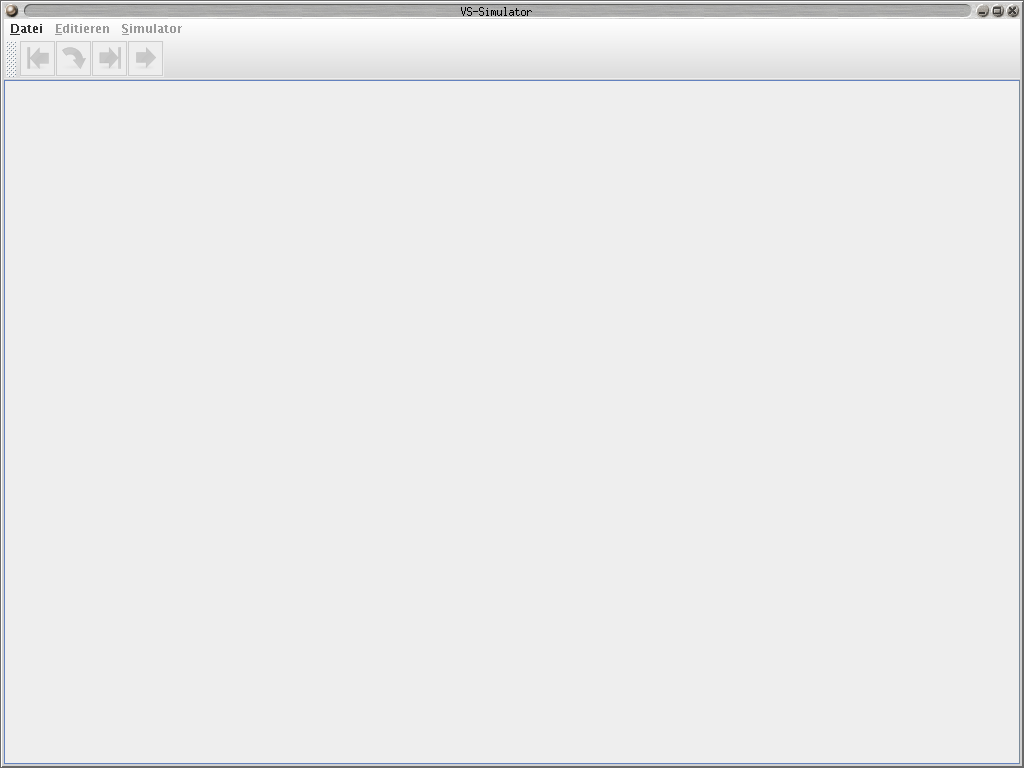
\includegraphics[width=12cm]{images/ss-neues-fenster}}
	\caption{Der Simulator nach dem ersten Starten}
	\label{fig:NeuesFenster}
\end{figure}

Der Simulator l\"{a}�t sich mit dem Befehl \textit{java -jar VS-Sim.jar} starten und pr\"{a}sentiert sich danach wie auf Abbildung \ref{fig:NeuesFenster}. F\"{u}r die Erstellung einer neuen Simulation wird im Men\"{u} ``Datei'' (Abbildung \ref{fig:DateiMenue}) der Punkt ``Neue Simulation'' ausgew\"{a}hlt, wo anschlie�end das Einstellungsfenster f\"{u}r die neue Simulation erscheint.  Auf die einzelnen Optionen wird sp\"{a}ter genauer eingegangen und es werden nun nur die Standardeinstellungen \"{u}bernommen. Die GUI mit einer frischen Simulation sieht aus wie auf Abbildung \ref{fig:NeuErstellteSimulation}.

\subsubsection{Die Men\"{u}zeile}

Im Datei-Men\"{u} (Abbildung \ref{fig:DateiMenue}) lassen sich neue Simulationen erstellen oder die aktuell ge\"{o}ffnete Simulation schlie�en. Neue Simulationen \"{o}ffnen sich standardm\"{a}�ig in einem neuen Tab. Es k\"{o}nnen allerdings auch neue Simulationsfenster, die wiederum eigene Tabs besitzen, ge\"{o}ffnet oder geschlossen werden. In jedem Tab befindet sich eine von den Anderen vollst\"{a}ndig unabh\"{a}ngige Simulation. Es k\"{o}nnen somit beliebig viele Simulationen parallel ausgef\"{u}hrt werden. Die Men\"{u}eintr\"{a}ge ``\"{O}ffnen'', ``Speichern'' und ``Speichern unter'' dienen f\"{u}r das Laden und Speichern von Simulationen. 

\begin{figure}[h]
	\centering
	\fbox{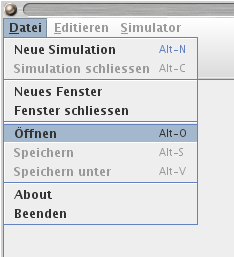
\includegraphics[width=6.5cm]{images/ss-datei-menu}}
	\caption{Datei-Men\"{u}}
	\label{fig:DateiMenue}
\end{figure}

\begin{figure}[h]
	\centering
	\fbox{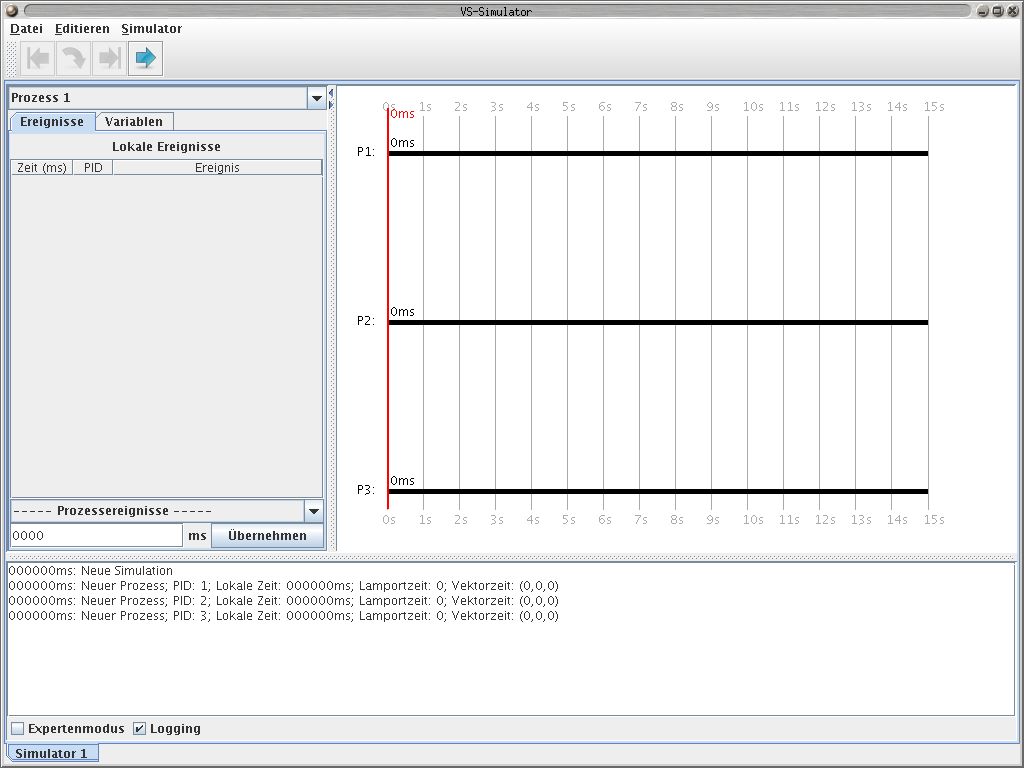
\includegraphics[width=12cm]{images/ss-neue-simulation}}
	\caption{Eine neue Simulation}
	\label{fig:NeuErstellteSimulation}
\end{figure}

\"{U}ber das Editieren-Men\"{u} gelangt der Anwender zu den Simulationseinstellungen, worauf sp\"{a}ter genauer eingegangen wird. In diesem Men\"{u} werden auch alle beteiligten Prozesse zum Editieren aufgelistet. W\"{a}hlt der Anwender dort einen Prozess aus, dann \"{o}ffnet sich der dazugeh\"{o}rige Prozesseditor. Auf diesen wird ebenso sp\"{a}ter genauer eingegangen. Das Simulator-Men\"{u} bietet die selben Optionen wie die Toolbar, welche im n\"{a}chsten Teilkapitel beschrieben wird, an.

Einige Men\"{u}unterpunkte sind erst erreichbar, wenn im aktuellen Fenster bereits eine Simulation erstellt oder geladen wurde.

\subsubsection{Die Toolbar}

Oben links im Simulator befindet sich die Toolbar (Abbildung \ref{fig:Toolbar}). Die Toolbar enth\"{a}lt die Funktionen die vom Anwender am h\"{a}ufigsten ben\"{o}tigt werden.

Die Toolbar bietet vier verschiedene Funktionen an:

\begin{figure}[h]
	\centering
	\fbox{
\includegraphics[width=5cm]{images/ss-neue-simulation-toolbar}}
	\caption{Die Men\"{u}zeile inklusive Toolbar}
	\label{fig:Toolbar}
\end{figure}

\begin{itemize}
	%\setlength{\itemsep}{-1mm}
	\item Zur\"{u}cksetzen der Simulation; kann nur bet\"{a}tigt werden, wenn die Simulation pausiert wurde oder wenn die Simulation abgelaufen ist.
	\item Wiederholen der Simulation; kann nicht bet\"{a}tigt werden, wenn die Simulation noch nicht gestartet wurde. 
	\item Pausieren der Simulation; kann nur bet\"{a}tigt werden, wenn die Simulation derzeit l\"{a}uft.
	\item Starten der Simulation; kann nur bet\"{a}tigt werden, wenn die Simulation derzeit nicht l\"{a}uft und noch nicht abgelaufen ist.
\end{itemize}

\newpage
\subsubsection{Die Visualisierung}

\begin{figure}[h]
	\centering
	\fbox{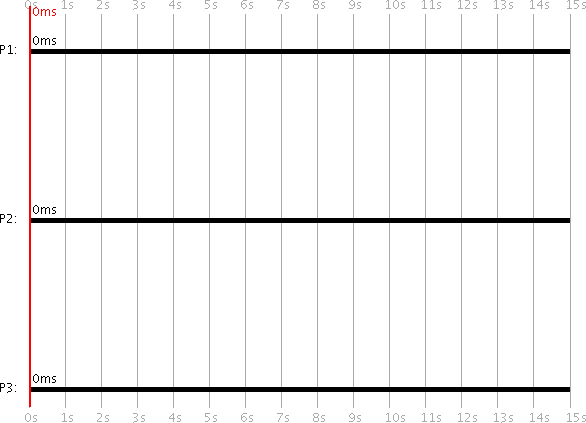
\includegraphics[width=12cm]{images/ss-visualisierung}}
	\caption{Visualisierung einer noch nicht gestarteten Simulation}
	\label{fig:Visualisierung}
\end{figure}

Mittig rechts befindet sich die grafische Simulationsvisualisierung. Die X-Achse gibt die Zeit in Millisekunden an und auf der Y-Achse sind alle beteiligten Prozesse aufgef\"{u}hrt. Die Demo-Simulation endet nach genau 15 Sekunden. Auf Abbildung \ref{fig:Visualisierung} sind 3 Prozesse (mit den PIDs 1, 2 und 3) dargestellt, die jeweils einen eigenen horizontalen schwarzen Balken besitzen. Auf diesen Prozessbalken kann der Anwender die jeweilige lokale Prozesszeit ablesen. Die vertikale rote Linie stellt die globale Simulationszeit dar. 

\begin{figure}[h]
	\centering
	\fbox{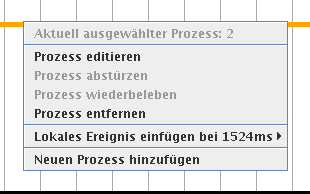
\includegraphics[width=8.8cm]{images/ss-rechtsklick-prozessbalken}}
	\caption{Rechtsklick auf einen Prozessbalken}
	\label{fig:RechtsklickProzessbalken}
\end{figure}

Die Prozessbalken dienen auch f\"{u}r Start- und Zielpunkte von Nachrichten. Wenn beispielsweise Prozess 1 eine Nachricht an Prozess 2 verschickt, so wird eine Linie vom einen Prozessbalken zum Anderen gezeichnet. Nachrichten, die ein Prozess an sich selbst verschickt, werden nicht visualisiert. Sie werden aber im Loggfenster (mehr dazu sp\"{a}ter) protokolliert.

Eine andere M\"{o}glichkeit einen Prozesseditor aufzurufen ist ein Linksklick auf den zum Prozess geh\"{o}rigen Prozessbalken. Dies muss also nicht immer \"{u}ber das Simulator-Men\"{u} geschehen. Ein Rechtsklick hingegen \"{o}ffnet ein Popup-Fenster mit weiteren Auswahlm\"{o}glichkeiten (Abbildung \ref{fig:RechtsklickProzessbalken}). Ein Prozess kann \"{u}ber das Popup-Men\"{u} nur w\"{a}hrend einer laufenden Simulation zu einem Absturz oder einer Wiederbelebung bewegt werden.

Generell kann die Anzahl der Prozesse nach belieben variieren. Die Dauer der Simulation betr\"{a}gt mindestens \textit{5} und h\"{o}chstens \textit{120} Sekunden. Die Simulation endet erst, wenn sie die globale Zeit die angegebene Simulationsendzeit (hier \textit{15} Sekunden) erreicht hat, und nicht, wenn eine lokale Prozesszeit diese Endzeit erreicht. 

\subsubsection{Farbliche Differenzierung}


Farben helfen dabei die Vorg\"{a}nge einer Simulation besser zu deuten. Standardm\"{a}�ig werden die Prozesse (Prozessbalken) und Nachrichten mit den Farben wie in Tabelle \ref{tb:Farben} aufgelistet dargestellt. Dies sind lediglich die Standardfarben, welche \"{u}ber die Einstellungen ge\"{a}ndert werden k\"{o}nnen.

\begin{table}
	\fbox{
	\begin{tabular}{c|l}
		\textbf{Prozessfarbe} & \textbf{Bedeutung} \\
		\hline 
		 	Schwarz & Die Simulation l\"{a}uft derzeit nicht\\
		\hline 
		 	Orange & Die Maus befindet sich \"{u}ber den Prozessbalken\\
		\hline 
		 	Rot & Der Prozess ist abgest\"{u}rzt\\
			& \\
		\textbf{Nachrichtenfarbe} & \textbf{Bedeutung} \\
		\hline 
		 	Gr\"{u}n & Die Nachricht ist noch unterwegs und hat das Ziel noch nicht erreicht\\
		\hline 
		 	Blau & Die Nachricht hat das Ziel erfolgreich erreicht\\
		\hline 
		 	Rot & Die Nachricht ging verloren\\
	\end{tabular}\\
	}
	\caption{Farbliche Differenzierung von Prozessen und Nachrichten}
	\label{tb:Farben}
\end{table}

\newpage
\subsubsection{Die Sidebar}

\begin{figure}[h]
	\centering
	\fbox{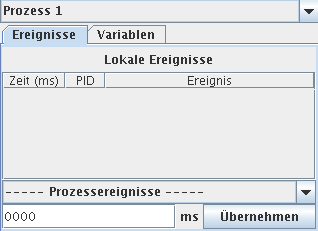
\includegraphics[width=9cm]{images/ss-sidebar}}
	\caption{Die Sidebar mit leerem Ereigniseditor}
	\label{fig:Sidebar}
\end{figure}

Mithilfe der Sidebar lassen sich Prozessereignisse programmieren. Oben auf Abbildung \ref{fig:Sidebar} ist der zu verwaltende Prozess selektiert (hier mit der PID 1). In dieser Prozessauswahl gibt es auch die M\"{o}glichkeit ``Alle Prozesse'' auszuw\"{a}hlen, womit die Ereignisse aller Prozesse gleichzeitig verwaltet werden k\"{o}nnen. Unter ``Lokale Ereignisse'' versteht man diejenigen Ereignisse, die auftreten, wenn eine bestimmte lokale Zeit des dazugeh\"{o}rigen Prozesses eingetreten ist. Die darunterliegende Ereignistabelle listet alle programmierten Ereignisse (hier noch keine vorhanden) mitsamt Eintrittszeiten sowie den PIDs auf.

\begin{figure}[h]
	\centering
	\fbox{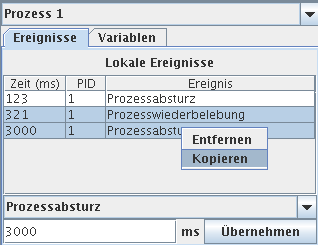
\includegraphics[width=9cm]{images/ss-sidebar-mit-ereignissen}}
	\caption{Der Ereigniseditor mit 3 programmierten Ereignissen}
	\label{fig:SidebarMitEreignissen}
\end{figure}

F\"{u}r die Erstellung eines neuen Ereignisses kann der Anwender entweder mit einem Rechtsklick auf einen Prozessbalken (Abbildung \ref{fig:RechtsklickProzessbalken}) klicken und dort ``Lokales Ereignis einf\"{u}gen'' w\"{a}hlen, oder unterhalb der Ereignistabelle ein Ereignis ausw\"{a}hlen (Abbildung \ref{fig:Ereignisauswahl}), im darunter liegenden Textfeld die Ereigniseintrittszeit eintragen und auf ``\"{U}bernehmen'' gehen. Beispielsweise wurden auf Abbildung \ref{fig:SidebarMitEreignissen} drei Ereignisse hinzugef\"{u}gt: Absturz nach \textit{123ms}, Wiederbelebung nach \textit{321ms} und erneuter Absturz nach \textit{3000ms} des Prozesses mit der ID 1. 

\begin{figure}[h]
	\centering
	\fbox{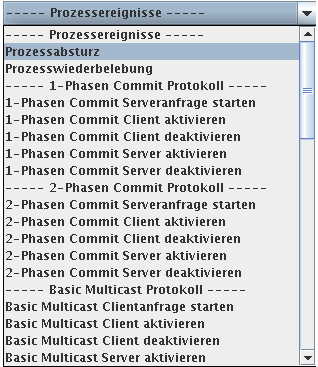
\includegraphics[width=9cm]{images/ss-ereignisauswahl}}
	\caption{Die Ereignisauswahl via Sidebar}
	\label{fig:Ereignisauswahl}
\end{figure}

Mit einem Rechtsklick auf den Ereigniseditor lassen sich alle selektierten Ereignisse entweder kopieren oder l\"{o}schen. Mithilfe der Strg-Taste k\"{o}nnen auch mehrere Ereignisse gleichzeitig markiert werden. Die Eintr\"{a}ge der Spalten f\"{u}r die Zeit und der PID lassen sich nachtr\"{a}glich editieren. Somit besteht eine komfortable M\"{o}glichkeit bereits programmierte Ereignisse auf eine andere Zeit zu verschieben oder einen anderen Prozess zuzuweisen. Allerdings sollte der Anwender darauf achten, dass er nach dem \"{A}ndern der Ereigniseintrittszeit die Enter-Taste bet\"{a}tigt, da sonst die \"{A}nderung unwirksam ist.

In der Sidebar gibt es neben dem Ereignis-Tab einen weiteren Tab ``Variablen''. Hinter diesem Tab verbirgt sich der Prozesseditor des aktuell ausgew\"{a}hlten Prozesses. Dort k\"{o}nnen alle Variablen des Prozesses editiert werden und ist somit eine weitere M\"{o}glichkeit einen Prozesseditor aufzurufen. Der Prozesseditor wird sp\"{a}ter genauer behandelt. 


\subsubsection{Das Loggfenster}

\begin{figure}[h]
	\centering
	\fbox{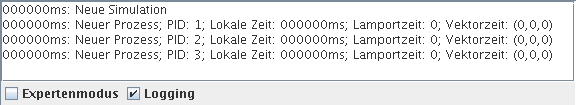
\includegraphics[width=16.5cm]{images/ss-loggfenster}}
	\caption{Das Loggfenster}
	\label{fig:Loggfenster}
\end{figure}

Das Loggfenster (Abbildung \ref{fig:NeuErstellteSimulation}, unten) protokolliert  in chronologischer Reihenfolge alle eingetroffenen Ereignisse. Auf Abbildung \ref{fig:Loggfenster} ist das Loggfenster nach Erstellung der Demo-Simulation zu sehen, an welcher 3 Prozesse beteiligt sind. Am Anfang eines Loggeintrages wird stets die globale Zeit in Millisekunden protokolliert. Bei jedem Prozess werden ebenso seine lokale Zeiten sowie die Lamport- und die Vektor-Zeitstempel aufgef\"{u}hrt. Letztere werden sp\"{a}ter genauer behandelt.  Hinter den Zeitangaben werden weitere Angaben, wie beispielsweise welche Nachricht mit welchem Inhalt verschickt wurde und welchem Protokoll sie angeh\"{o}rt, gemacht. Dies wird sp\"{a}ter noch anhand von Beispielen demonstriert.

Mit dem Deaktivieren des Logging-Schalters l\"{a}�t sich das Loggen von Nachrichten tempor\"{a}r ausstellen. Mit deaktiviertem Loggen werden keine neuen Nachrichten mehr ins Loggfenster geschrieben. Nach Reaktivieren des Schalters werden alle ausgelassenen Nachrichten nachtr\"{a}glich in das Fenster geschrieben. Ein deaktiviertes Loggen kann zu verbessertem Leistungsverhalten des Simulators f\"{u}hren (z.B. kein Rucklen; ist vom verwendeten Computer, auf dem der Simulator l\"{a}uft, abh\"{a}ngig). Dieser Umstand ist der sehr langsamen Java-Implementierung der JTextArea-Klasse zu verdanken, die schnelle Updates nur sehr tr\"{a}ge durchf\"{u}hrt.

\"{U}ber den Schalter ``Expertenmodus'' wird der Expertenmodus aktiviert beziehungsweise deaktiviert. 

\section{Expertenmodus}

\begin{figure}[h]
	\centering
	\fbox{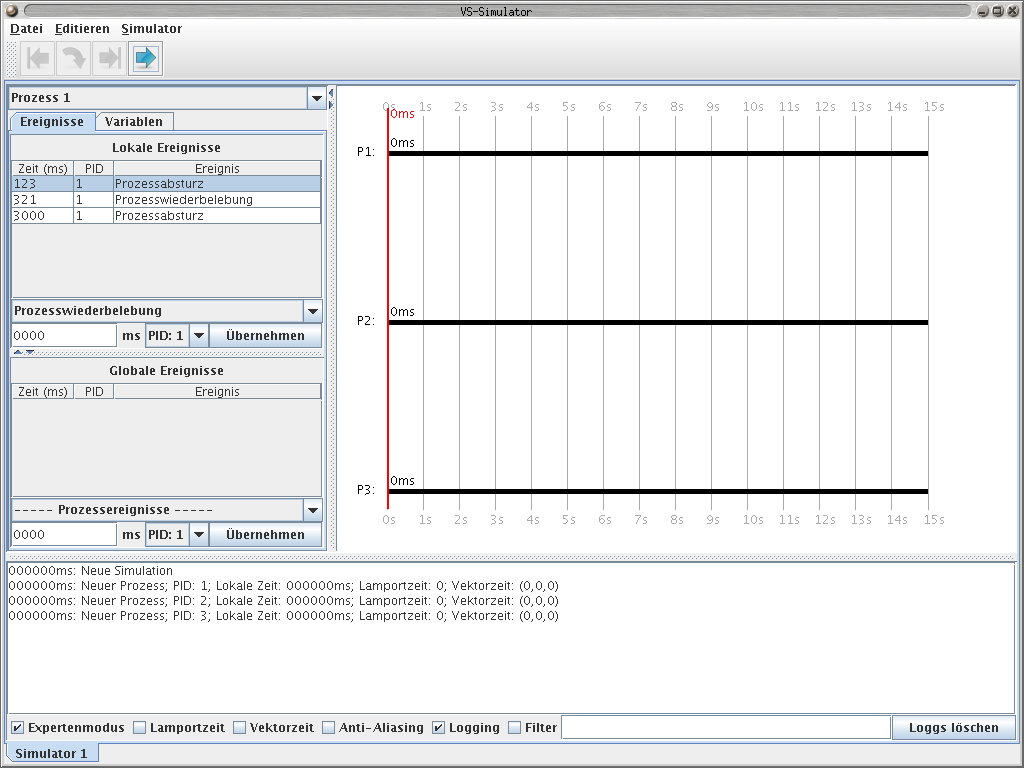
\includegraphics[width=12cm]{images/ss-simulation-expertenmodus}}
	\caption{Der Simulator im Expertenmodus}
	\label{fig:SimulationExpertenmodus}
\end{figure}

Der Simulator kann in zwei verschiedenen Modi betrieben werden. Es gibt einen einfachen- und einen Expertenmodus. Der Simulator startet standardm\"{a}�ig im einfachen Modus, sodass sich der Anwender nicht mit der vollen Funktionalit\"{a}t des Simulators auf einmal auseinandersetzen mu�. Der einfache Modus ist \"{u}bersichtlicher, bietet jedoch weniger Funktionen an. Der Expertenmodus eignet sich mehr f\"{u}r erfahrene Anwender und bietet dementsprechend auch mehr Flexibilit\"{a}t. Der Expertenmodus kann \"{u}ber den gleichnamigen Schalter unterhalb des Loggfensters oder \"{u}ber die Simulationseinstellungen aktiviert oder deaktiviert werden.  Auf Abbildung \ref{fig:SimulationExpertenmodus} ist der Simulator im Expertenmodus zu sehen. Wenn der Expertenmodus mit dem normalen Modus verglichen wird, dann fallen einige Unterschiede auf:

\subsubsection{Neue Funktionen in der Sidebar}

Der erste Unterschied ist in der Sidebar erkennbar (Abbildung \ref{fig:SidebarExpertenmodus}). Dort sind nun, zus\"{a}tzlich den lokalen Ereignissen, auch globale Ereignisse editierbar.  Wie bereits erw\"{a}hnt sind unter lokale Ereignisse diejenigen Ereignisse zu verstehen, die auftreten, wenn eine bestimmte lokale Zeit des dazugeh\"{o}rigen Prozesses eingetreten ist. Globale Ereignisse hingegen sind diejenigen Ereignisse, die auftreten, wenn eine bestimmte globale Zeit eingetreten ist. Ein globales Ereignis nimmt die globale Zeit- und ein lokales Ereignis die lokale Prozesszeit als Eintrittskriterium. Globale Ereignisse machen somit nur einen Unterschied, wenn sich die lokalen Prozesszeiten von der globalen Zeit unterscheiden.

Des Weiteren kann der Anwender bei der Programmierung eines neuen Ereignisses direkt die dazugeh\"{o}rige PID selektieren. Im einfachen Modus wurde hier immer standardm\"{a}�ig die PID des aktuell (in der obersten Combo-Box) ausgew\"{a}hlten Prozesses verwendet (hier mit PID 1). In dieser Combo-Box sollte der Anwender gegebenenfalls ``Alle Prozesse'' selektieren, damit im Ereigniseditor stets die Ereignisse aller Prozesse aufgelistet werden.

\subsubsection{Lamportzeit-, Vektorzeit- und Anti-Aliasing Schalter}

Weitere Unterschiede machen sich unterhalb des Loggfensters bemerkbar. Dort gibt es unter Anderem zwei neue Schalter ``Lamportzeit'' und ``Vektorzeit''.  Aktiviert der Anwender einen dieser beiden Schalter, so wird die Lamport- beziehungsweise Vektorzeit in der Visualisierung dargestellt. Damit die \"{U}bersichtlichkeit nicht leidet, kann der Anwender nur jeweils einen dieser beiden Schalter zur gleichen Zeit aktiviert haben. 

\begin{figure}[h]
	\centering
	\fbox{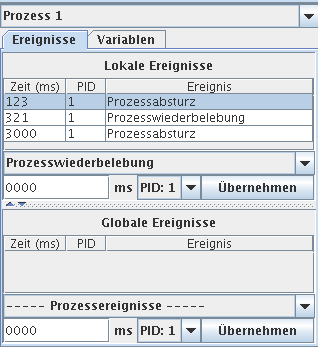
\includegraphics[width=9cm]{images/ss-sidebar-expertenmodus}}
	\caption{Die Sidebar im Expertenmodus}
	\label{fig:SidebarExpertenmodus}
\end{figure}

Der Anti-Aliasing-Schalter erm\"{o}glicht dem Anwender Anti-Aliasing zu aktivieren beziehungsweise zu deaktivieren. Mit Anti-Aliasing werden alle Grafiken der Visualisierung gerundet dargestellt. Aus Performancegr\"{u}nden ist Anti-Aliasing standardm\"{a}�ig nicht aktiv.

\subsubsection{Der Loggfilter}

Je komplexer eine Simulation wird, desto un\"{u}bersichtlicher werden die Eintr\"{a}ge im Loggfenster. Hier f\"{a}llt es zunehmend schwerer die \"{U}bersicht aller Ereignisse zu behalten. Um dem entgegenzuwirken gibt es im Expertenmodus einen Loggfilter, welcher es erm\"{o}glicht nur die wesentlichen Daten aus den Loggs zu filtern. 

Der Loggfilter wird anhand dem dazugeh\"{o}rigen Schalter ``Filter'' aktiviert und deaktiviert. In der dahinterliegenden Eingabezeile kann ein regul\"{a}rer Ausdruck in Java-Syntax angegeben werden. Beispielsweise werden mit ``\textit{PID: (1|2)}'' nur Loggzeilen angezeigt, die entweder ``\textit{PID: 1}'' oder ``\textit{PID: 2}'' beinhalten. Alle anderen Zeilen, die zum Beispiel nur ``\textit{PID: 3}'' beinhalten, werden dabei nicht angezeigt. Mit Loggfilter werden nur die Loggzeilen angezeigt, auf die der angegebene regul\"{a}re Ausdruck passt. Der Loggfilter kann auch nachtr\"{a}glich aktiviert werden, da bereits protokollierte Ereignisse nach jeder Filter\"{a}nderung erneut gefiltert werden. 

Der Loggfilter kann auch w\"{a}hrend einer laufenden Simulation verwendet werden. Bei Filterdeaktivierung werden alle Nachrichten wieder dargestellt. Loggnachrichten, die aufgrund des Filters noch nie angezeigt wurden, werden dann nachtr\"{a}glich angezeigt.

\section{Ereignisse}

Es wird zwischen zwei Haupttypen von Ereignissen unterschieden: Programmierbare Ereignisse und nicht programmierbare Ereignisse. Programmierbare Ereignisse lassen sich im Ereigniseditor programmieren und editieren und deren Eintrittszeiten h\"{a}ngen von den lokalen Prozessuhren oder der globalen Uhr ab. Nicht-programmierbare Ereignisse lassen sich hingegen nicht im Ereigniseditor programmieren und treten nicht wegen einer bestimmten Uhrzeit ein, sondern aufgrund anderer Gegebenheiten wie zum Beispiel das Eintreffen einer Nachricht oder das Ausf\"{u}hren einer Aktion aufgrund eines Weckers, worauf sp\"{a}ter nochmal genauer eingegangen wird.

\subsubsection{Prozessabsturz- und Wiederbelebung (programmierbar)}

Die beiden einfachsten Ereignisse sind ``Prozessabsturz'' sowie ``Prozesswiederbelebung''. Wenn ein Prozess abgest\"{u}rzt ist, so wird sein Prozessbalken in rot dargestellt. Ein abgest\"{u}rzter Prozess kann keine weiteren Ereignisse mehr verarbeiten und wenn bei ihm eine Nachricht eintrifft, dann kann sie nicht verarbeitet werden und geht deshalb verloren. Die einzige Ausnahme bildet ein Wiederbelebungsereignis. Ein abgest\"{u}rzter Prozess kann nichts, au�er wiederbelebt werden. W\"{a}hrend eines Prozessabsturzes l\"{a}uft die lokale Prozessuhr, abgesehen der Lamport- und Vektor-Uhren, normal weiter. Das hei�t es besteht die M\"{o}glichkeit, dass ein Prozess einige seiner Ereignisse gar nicht ausf\"{u}hrt, da er zu den Ereigniseintrittszeiten abgest\"{u}rzt ist. Wenn im echten Leben ein Computer abst\"{u}rzt oder abgeschaltet wird, dann l\"{a}uft seine Hardware-Uhr unabh\"{a}ngig vom Betriebssystem auch weiter.

\subsubsection{Aktivierung und Deaktivierung von Protokollen sowie Starten von Anfragen (programmierbar)}
Es ist bereits bekannt, dass ein Prozess mehrere Protokolle client- und auch serverseitig unterst\"{u}tzen kann. Welches Protokoll von einem Prozess unterst\"{u}tzt wird, kann der Anwender anhand von Protokollaktivierungs- und Protokolldeaktivierungsereignissen konfigurieren. Somit besteht die M\"{o}glichkeit, dass ein gegebener Prozess ein bestimmtes Protokoll erst zu einem bestimmten Zeitpunkt unterst\"{u}tzt und gegebenenfalls ein anderes Protokoll abl\"{o}st. Jedes Protokoll kann entweder server- oder clientseitig aktiviert beziehungsweise deaktiviert werden. Welche Protokolle es gibt wird sp\"{a}ter behandelt. Der Anwender hat somit die Auswahl zwischen f\"{u}nf verschiedenen Protokollereignistypen: 

\begin{itemize}
	\item Aktivierung des Clients eines gegebenen Protokolls
	\item Aktivierung des Servers eines gegebenen Protokolls
	\item Deaktivierung des Clients eines gegebenen Protokolls
	\item Deaktivierung des Servers eines gegebenen Protokolls
	\item Starten einer Client/Server-Anfrage eines gegebenen Protokolls
\end{itemize}

Ob sich das Ereignis f\"{u}r das Starten einer Anfrage auf einen Client oder einen Server bezieht h\"{a}ngt vom verwendeten Protokoll ab. Es gibt Protokolle, wo der Client die Anfragen starten muss, und es gibt Protokolle, wo der Server diese Aufgabe \"{u}bernimmt. Beispielsweise startet bei dem ``Ping-Pong Protokoll'' der Client- und bei dem ``Commit-Protokollen'' der Server immer die Anfragen. Es gibt kein Protokoll, wo der Client und der Server jeweils Anfragen starten k\"{o}nnen. 

\subsubsection{Nachrichtenempfang sowie Antwortnachrichten (nicht-programmierbar)}

Nachdem ein Prozess eine Nachricht empf\"{a}ngt wird zuerst \"{u}berpr\"{u}ft, ob er das dazugeh\"{o}rige Protokoll unterst\"{u}tzt. Wenn der Prozess das Protokoll unterst\"{u}tzt wird geschaut, ob es sich um eine Client- oder eine Servernachricht handelt. Wenn es sich um eine Clientnachricht handelt, so mu� der Empf\"{a}ngerprozess das Protokoll serverseitig unterst\"{u}tzen und virce versa. Wenn alles passt, dann f\"{u}hrt der Empf\"{a}ngerprozess die vom Protokoll definierten Aktionen aus. In der Regel berechnet der Prozess einen bestimmten Wert und schickt ihn \"{u}ber eine Antwortnachricht zur\"{u}ck. Es k\"{o}nnen aber auch beliebig andere Aktionen ausgef\"{u}hrt werden. Welche dies sind h\"{a}ngt vom Protokoll ab.

\subsubsection{Callback-Ereignisse (nicht-programmierbar)}

Ein Callback-Ereignis kann von einem Protokoll ausgel\"{o}st werden. Das Protokoll setzt einen Wecker, der angibt zur welcher lokalen Uhrzeit eine weitere Aktion ausgef\"{u}hrt werden soll. Zum Beispiel lassen sich hiermit Timeouts realisieren: Wenn ein Protokoll eine Antwort erwartet, diese aber nicht eintrifft, dann kann nach einer bestimmten Zeit eine Anfrage erneut verschickt werden! Es k\"{o}nnen beliebig viele Callback-Ereignisse definiert werden. Wenn sie noch nicht ausgef\"{u}hrt wurden und aufgrund eines anderen Ereignisses nicht mehr ben\"{o}tigt werden, dann k\"{o}nnen sie vom Protokoll wieder nachtr\"{a}glich entfernt werden. Wenn ein Callback-Ereignis ausgef\"{u}hrt wird, dann kann es sich selbst wieder f\"{u}r eine weitere Ausf\"{u}hrung erneut planen. So lassen sich periodisch wieder-eintreffende Ereignisse realisieren. Beispielsweise verwenden die ``Commit-Protokolle'' (mehr dazu sp\"{a}ter) Callback-Ereignisse, indem solange Anfragen verschickt werden, bis alle ben\"{o}tigten Antworten vorliegen.

\subsubsection{Zufallsereignisse (nicht-programmierbar)}

Die Eintrittszeit eines Zufallsereignisses wird vom Simulator zuf\"{a}llig gew\"{a}hlt. Es besteht lediglich die M\"{o}glichkeit die Wahrscheinlichkeit, dass das Ereignis \"{u}berhaupt eintritt, einzustellen. Ein Beispiel ist ein zuf\"{a}lliger Prozessabsturz, dessen Wahrscheinlichkeit unter den Prozessvariablen konfiguriert werden kann. Diese Variable wird im Abschnitt \"{u}ber den Prozesseditor noch ausf\"{u}hrlicher beschrieben.


\section{Einstellungen}

\begin{table}
	\centering
	\fbox{
	\begin{tabular}{l|l}
		\textbf{Typ} & \textbf{Beschreibung}\\
		\hline 
			\textit{Boolean} & Boolscher Wert, z.B. \textit{true} oder \textit{false}\\
			\textit{Color} & Java-Farbobjekt\\
			\textit{Float} & 32-Bit Flie�kommazahl\\
			\textit{Integer[]} & Vektor aus 32-Bit Integern\\
			\textit{Integer} & 32-Bit Integer\\
			\textit{Long} & 64-Bit Long\\
			\textit{String} & Java-Stringobjekt\\
	\end{tabular}
	}
	\caption{Verf\"{u}gbare Datentypen f\"{u}r editierbare Variablen}
	\label{tb:VariablenDatentypen}
\end{table}


In diesem Abschnitt wird genauer auf die m\"{o}glichen Konfigurationsm\"{o}glichkeiten eingegangen. Zun\"{a}chst gibt es globale Simulationseinstellungen. Diese beinhalten Variablen die die gesamte Simulation betreffen. Zudem hat jeder Prozess seine eigenen lokale Einstellungen. Dar\"{u}ber hinaus kann jedes Protokoll (Client- sowie Serverseite) f\"{u}r jeden Prozess separat eingestellt werden. 

\subsection{Variablendatentypen}

\begin{figure}[h]
	\centering
	\fbox{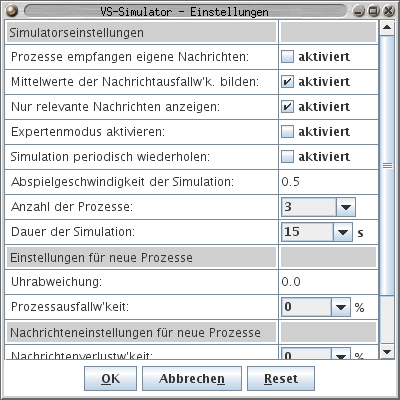
\includegraphics{images/ss-simulationseinstellungen}}
	%\fbox{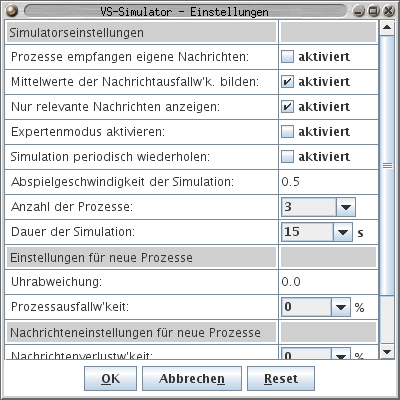
\includegraphics[width=11cm]{images/ss-simulationseinstellungen}}
	\caption{Das Fenster zu den Simulationseinstellungen}
	\label{fig:Simulationseinstellungen}
\end{figure}


Der Simulator unterscheidet zwischen mehreren Datentypen, in denen die einstellbaren Variablen vorliegen k\"{o}nnen (Tabelle \ref{tb:VariablenDatentypen}). Jede Variable besitzt einen Namen, einen Wert und eine optionale Beschreibung. Wenn eine Variablenbeschreibung vorhanden ist, so wird sie anstelle des Variablennamen in einem Editor (mehr zu Editoren sp\"{a}ter) angezeigt. Der Variablenname wird vom Simulator lediglich f\"{u}r die interne Verwendung ben\"{o}tigt. Im folgenden bedeutet \textit{Typ: varname = wert}, dass die Variable vom Typ \textit{Typ} ist, der interne Variablenname \textit{varname} lautet, und standardm\"{a}ssig den Wert \textit{wert} zugewiesen hat. Vom Anwender lassen sich lediglich die Variablenwerte, jedoch nicht die Variablentypen, Variablennamen und Beschreibungen, \"{a}ndern.

\subsection{Simulationseinstellungen}


Beim Erstellen einer neuen Simulation erscheint zun\"{a}chst das dazugeh\"{o}rige Einstellungsfenster (Abbildung \ref{fig:Simulationseinstellungen}). In der Regel reicht es, wenn der Anwender hier, bis auf die Anzahl beteiligter Prozesse, die Standardwerte \"{u}bernimmt. Es besteht auch die M\"{o}glichkeit die Einstellungen nachtr\"{a}glich zu editieren, indem das Einstellungsfenster via ``Editieren $\rightarrow$ Einstellungen'' erneut aufgerufen wird.

Im Folgenden werden alle in den Simulationseinstellungen verf\"{u}gbaren Variablen beschrieben. Die Klammern geben die Typen, Namen und die Standardwerte an, in denen die Variablen vorliegen. 

\begin{figure}[h]
	\centering
	\fbox{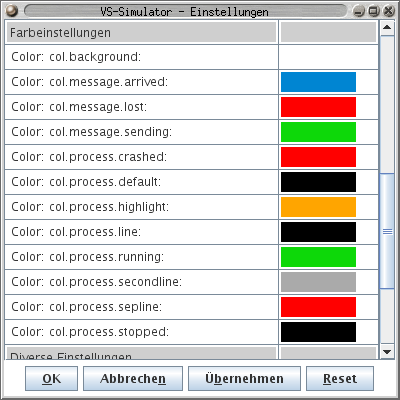
\includegraphics{images/ss-simulationseinstellungen-experten}}
	\caption{Weitere Simulationseinstellungen im Expertenmodus}
	\label{fig:SimulationseinstellungenExperten}
\end{figure}


\begin{itemize}
	\item \textbf{Prozesse empfangen eigene Nachrichten} \textit{(Boolean: sim.message.own.recv = false)}: Standardm\"{a}�ig k\"{o}nnen Prozesse keine Nachrichten empfangen, die sie selbst verschickt haben. Dies tr\"{a}gt zur \"{U}bersichtlichkeit der Simulation bei. Wenn diese Variable jedoch auf \textit{true} gesetzt wird, dann kann ein Prozess auch selbst verschickte Nachrichten emfpangen und auf diese ebenso antworten. Die Zeit f\"{u}r das Versenden und Empfangen einer Nachricht an sich selbst betr\"{a}gt jedoch stets \textit{0ms}. Diese Variable sollte mit Vorsicht verwendet werden, da bedingt durch den \textit{0ms} Endlosschleifen entstehen k\"{o}nnen. 
	\item \textbf{Mittelwerte der Nachrichtenverlustwahrscheinlichkeiten bilden} \textit{(Boolean: sim.message.prob.mean = true)}: Jede Nachricht die verschickt wird hat, je nach Einstellungen, eine vom verschickenden Prozess abh\"{a}ngige zuf\"{a}llige Verlustwahrscheinlichkeit. Wenn diese Option aktiviert ist, so wird die der Mittelwert aus den Verlustwahrscheinlichkeiten vom Sender- und Empf\"{a}ngerprozess gebildet. Ansonsten wird stets die Verlustwahrscheinlichkeit, die beim Senderprozesses angegeben wurde, verwendet. 
	\item \textbf{Mittelwerte der \"{U}bertragungszeiten bilden} \textit{(Boolean: sim.message.sendingtime.mean = true)}: Jede Nachricht die verschickt wird hat, je nach Einstellungen, eine vom verschickenden Prozess abh\"{a}ngige zuf\"{a}llige \"{U}bertragungszeit bis sie ihr Ziel erreicht (siehe Prozesseinstellungen sp\"{a}ter). Wenn diese Option aktiviert ist, so wird der Mittelwert vom Sender- und Empf\"{a}ngerprozess gebildet. Ansonsten wird stets die \"{U}bertragungszeit, die beim Senderprozesses angegeben wurde, verwendet.
	\item \textbf{Nur relevante Nachrichten anzeigen} \textit{(Boolean: sim.messages.relevant = true)}: Wenn nur alle relevanten Nachrichten angezeigt werden, dann werden Nachrichten an einen Prozess die er selbst nicht verarbeiten kann, weil er das dazugeh\"{o}rige Protokoll nicht unterst\"{u}tzt, nicht angezeigt. Dies verbessert die \"{U}bersicht.
	\item \textbf{Expertenmodus aktivieren} \textit{(Boolean: sim.mode.expert = false)}: Hier l\"{a}sst sich der Expertenmodus aktivieren beziehungsweise deaktivieren. Alternativ kann dies \"{u}ber den gleichnamigen Schalter unterhalb des Loggfensters geschehen.
	\item \textbf{Simulation periodisch wiederholen} \textit{(Boolean: sim.periodic = false)}: Wenn diese Variable auf \textit{true} gesetzt ist, dann wird die Simulation jedes Mal nach Ablauf automatisch erneut gestartet. 
	\item \textbf{Lamportzeiten betreffen alle Ereignisse} \textit{(Boolean: sim.update.lamporttime.all = false)}: Wenn diese Variable auf \textit{true} gesetzt ist, dann werden bei jedem Ereignis alle Lamportzeitstempel aller Prozesse jeweils inkrementiert. Bei einem Wert \textit{false} inkrementieren sich die Lamportzeitstempel jeweils nur, wenn eine Nachricht empfangen oder verschickt wurde.
	\item \textbf{Vektorzeiten betreffen alle Ereignisse} \textit{(Boolean: sim.update.vectortime.all = false)}: Wenn diese Variable auf \textit{true} gesetzt ist, dann werden bei jedem Ereignis alle Vektor-Zeitstempel aller Prozesse jeweils inkrementiert. Bei einem Wert \textit{false} inkrementieren sich die Vektor-Zeitstempel jeweils nur, wenn eine Nachricht empfangen oder verschickt wurde.

	Lamport- und Vektorzeitstempel werden sp\"{a}ter anhand eines Beispiels verdeutlicht.
	\item \textbf{Abspielgeschwindigkeit der Simulation} \textit{(Float: sim.clock.speed = 0.5)}: Gibt den Faktor der Simulationsabspielgeschindigkeit an. Wenn als Faktor \textit{1} gew\"{a}hlt wird, dann dauert eine simulierte Sekunde so lange wie eine echte Sekunde. Der Faktor \textit{0.5} gibt somit an, dass die Simulation mit halber Echtzeitgschwindigkeit abgespielt wird.
	\item \textbf{Anzahl der Prozesse} \textit{(Integer: sim.process.num = 3)}: Gibt die Anzahl beteiligter Prozesse an. Der Anwender kann auch nachtr\"{a}glich via Rechtsklick auf den Prozessbalken den jeweiligen Prozess aus der Simulation entfernen oder weitere Prozesse hinzuf\"{u}gen.
	\item \textbf{Dauer der Simulation} \textit{(Integer: sim.seconds = 15)}: Gibt die Dauer der Simulation in Sekunden an.
\end{itemize}

Die weiteren Simulationseinstellungen unter ``Einstellungen f\"{u}r neue Prozesse'' sowie ``Nachrichteneinstellungen f\"{u}r neue Prozesse'' geben lediglich Standardwerte an, die f\"{u}r neu zu erstellende Prozesse verwendet werden. Die dort verf\"{u}gbaren Variablen werden im folgenden Teilkapitel genauer beschrieben.

\subsection{Prozess- und Protokolleinstellungen}

Jeder Prozess besitzt folgende Variablen, die entweder via dem Variablen-Tab in der Sidebar oder ``Editieren $\rightarrow$ Prozess \textit{PID}'' oder Linksklick auf den Prozessbalken editiert werden k\"{o}nnen. Auf allen drei Wegen kommt jeweils der selbe Prozesseditor zum Vorschein.

\begin{itemize}
	\item \textbf{Uhrabweichung} \textit{(Float: process.clock.variance = 0.0)}: Gibt den Wert an, um den die lokale Prozessuhr abweicht. Der Wert \textit{0.0} besagt beispielsweise, dass die Uhr keine Abweichung hat und somit global-korrekt l\"{a}uft. Ein Wert von \textit{1.0} w\"{u}rde hingegen bedeuten, dass die Uhr mit doppelter Geschwindigkeit- und ein Wert von \textit{-0.5}, dass die lokale Prozessuhr mit halber Geschwindigkeit der globalen Uhr fortschreitet. Es sind nur Werte > \textit{-1.0} erlaubt, da sonst die Prozessuhr r\"{u}ckw\"{a}rts laufen k\"{o}nnte. Bei allen anderen Werten wird die Einstellung wieder automatisch auf \textit{0.0} gesetzt. Da der Simulator intern mit Flie�kommazahlen doppelter Genauigkeit arbeitet, kann es zu kleinen, jedoch vernachl\"{a}ssigbaren, Rundungsfehlern kommen. 
	\item \textbf{Prozessausfallwahrscheinlichkeit} \textit{(Integer: process.prob.crash = 0)}: Gibt eine Wahrscheinlichkeit in Prozent an, ob der gegebene Prozess w\"{a}hrend der Simulation zuf\"{a}llig abst\"{u}rzt. Die Wahrscheinlichkeit bezieht sich auf die komplette Simulationsdauer. Bei einer Einstellung von \textit{100} Prozent und der Simulationsdauer von \textit{15} Sekunden st\"{u}rzt der Prozess auf jeden Fall zwischen \textit{0ms} und \textit{15000ms} ab. An welcher Stelle dies geschieht wird zuf\"{a}llig bestimmt. Wenn der Prozess nach seinem Absturz wiederbelebt wird, st\"{u}rzt er nicht noch einmal zuf\"{a}llig ab. Dies gilt allerdings nicht, wenn die Prozesseinstellungen nach dem Zufallsabsturz erneut ge\"{a}ndert und \"{u}bernommen werden, da dann das Zufallsabst\"{u}rzereignis erneut erstellt wird. 
	\item \textbf{Lokale Zeit} \textit{(Long: process.localtime = 0)}: Gibt die lokale Prozesszeit in Millisekunden an. 
	\item \textbf{Nachrichtenverlustwahrscheinlichkeit} \textit{(Integer: message.prob.crash = 0)}: Gibt eine Wahrscheinlichkeit in Prozent an, ob eine vom aktuell ausgew\"{a}hlten Prozess verschickte Nachricht unterwegs verloren geht. An welcher Stelle die Nachricht zwischen dem Sende- und Empfangsprozess verloren geht wird vom Simulator zuf\"{a}llig gew\"{a}hlt.
	\item \textbf{Maximale \"{U}bertragungszeit} \textit{(Long: message.sendingtime.max = 2000)}: Gibt die Dauer in Millisekunden an, die eine vom Prozess verschickte Nachricht maximal ben\"{o}tigt, bis sie einen Empf\"{a}ngerprozess erreicht. Im weiteren Verlauf wird dieser Wert mit $t_{max}$ bezeichnet. 
	\item \textbf{Minimale \"{U}bertragungszeit} \textit{(Long: message.sendingtime.min = 500)}: Gibt die Dauer in Millisekunden an, die eine vom Prozess verschickte Nachricht minimal ben\"{o}tigt, bis sie einen Empf\"{a}ngerprozess erreicht. Im weiteren Verlauf wird dieser Wert mit $t_{min}$ bezeichnet. 
		
Wenn die \"{U}bertragungszeiten von Nachrichten immer exakt die selbe Zeit in Anspruch nehmen sollen, dann m\"{u}ssen alle Prozesseinstellungen mit $t_{min} = t_{max}$ konfiguriert werden. Wenn die aktuelle globale Zeit $t_g$ ist und die Simulationseinstellung ``Mittelwerte der \"{U}bertragungszeiten'' nicht aktiv ist, dann wird die Ereigniseintrittszeit $t_e$ f\"{u}r den Empfang der Nachricht wie folgt berechnet:

\begin{equation*}
	t_e := t_g + rand(t_{min}, t_{max})
\end{equation*}

Das hei�t, dass die Nachricht nach einer zuf\"{a}lligen Zeit zwischen $t_{min}$ und $t_{max}$ beim Empf\"{a}nger eintrifft. F\"{u}r jeden Emfp\"{a}nger wird hierbei ein neuer Zufallswert gew\"{a}hlt. F\"{u}r den Fall, dass die Einstellung ``Mittelwerte der \"{U}bertragungszeiten w\"{a}hlen'' aktiviert ist, und wenn $t'_{min}$ und $t'_{max}$ die beim Empf\"{a}ngerprozess eingestellten Werte ensprechen, dann wird die Nachrichtenempfangszeit wie folgt berechnet:

\begin{equation*}
	t_e := t_g + \frac{1}{2} (rand(t_{min}, t_{max}) + rand(t'_{min}, t'_{max}))
\end{equation*}

Das hei�t, dass stets der Mittelwert der Nachrichten\"{u}bertragungszeiten des Sender- und Empf\"{a}ngerprozesses verwendet wird.

\end{itemize}

Im selben Fenster lassen sich auch die Protokollvariablen editieren. Die Protokollvariablen werden jedoch sp\"{a}ter bei den Protokollen beschrieben.

\subsection{Einstellungen im Expertenmodus}

\begin{table}
	\centering
	\fbox{
	\begin{tabular}{l|l}
		\textbf{Schl\"{u}ssel} & \textbf{Beschreibung}\\
		\hline 
			\textit{col.background} & Die Hintergrundfarbe der Simulation\\
			\textit{col.message.arrived} & Nachrichtenfarbe wenn sie ihr Ziel erreicht hat\\
			\textit{col.message.lost} & Nachrichtenfarbe wenn sie verloren ging\\
			\textit{col.message.sending} & Nachrichtenfarbe wenn sie noch unterwegs ist\\
			\textbf{\textit{col.process.crashed}} & Prozessfarbe wenn er abgest\"{u}rzt ist\\
			\textbf{\textit{col.process.default}} & Prozessfarbe wenn die Simulation aktuell nicht l\"{a}uft und \\
				& der Prozess aktuell nicht abgest\"{u}rzt ist \\
			\textbf{\textit{col.process.highlight}} & Prozessfarbe wenn die Maus \"{u}ber seinem Balken liegt\\
			\textit{col.process.line} & Farbe, in der die kleine ``Prozessfane'' an der auch die \\
				& lokale Prozesszeit angegeben wird, dargestellt wird\\
			\textbf{\textit{col.process.running}} & Prozessfarbe wenn er nicht abgest\"{u}rzt ist und die\\
				& Simulation aktuell l\"{a}uft\\
			\textit{col.process.secondline} & Farbe in der die Sekunden-Zeitgitter dargestellt werden \\
			\textit{col.process.sepline} & Farbe der globalen Zeitachse\\
			\textbf{\textit{col.process.stopped}} & Prozessfarbe wenn die Simulation pausiert wurde\\
	\end{tabular}
	}
	\caption{Farbeinstellungen}
	\label{tb:Farbeinstellungen}
\end{table}

Im Expertenmodus lassen sich zus\"{a}tzliche Variablen, wie beispielsweise diverse Farbwerte und Anzahl oder Pixel verschiedener der GUI-Elemente, editieren. Auf Abbildung \ref{fig:SimulationseinstellungenExperten} sieht der Anwender alle einstellbaren Farben. Die fett-gedruckten Schl\"{u}ssel in Tabelle \ref{tb:Farbeinstellungen} dienen nur als Standardwerte f\"{u}r die neu zu erstellenen Prozesse und sind auch jeweils in den Prozesseinstellungen f\"{u}r jeden Prozess separat editierbar.

\section{Protokolle}

Im Folgenden werden alle verf\"{u}gbaren Protokolle behandelt. Wie bereits beschrieben wird bei Protokollen zwischen Server- und Clientseite unterschieden. Server k\"{o}nnen auf Clientnachrichten, und Client auf Servernachrichten antworten. Jeder Prozess kann beliebig viele Protokolle sowohl clientseitig als auch serverseitig unterst\"{u}tzen. Theoretisch ist es auch m\"{o}glich, dass ein Prozess f\"{u}r ein bestimmtes Protokoll gleichzeitig der Server und der Client ist. Der Anwender kann auch weitere eigene Protokolle in der Programmiersprache Java mittels einer speziellen API (Application Programming Interface) erstellen. Wie eigene Protokolle erstellt werden k\"{o}nnen wird sp\"{a}ter behandelt. 

\subsection{Beispiel (Dummy) Protokoll}

Das Dummy-Protokoll dient lediglich als leeres Template f\"{u}r die Erstellung eigener Protokolle. Bei der Verwendung des Dummy-Protokolls werden bei Ereignissen lediglich Loggnachrichten ausgegeben. Es werden aber keine weiteren Aktionen ausgef\"{u}hrt.

\newpage
\subsection{Das Ping-Pong Protokoll}

\begin{figure}[h]
	\centering
	\fbox{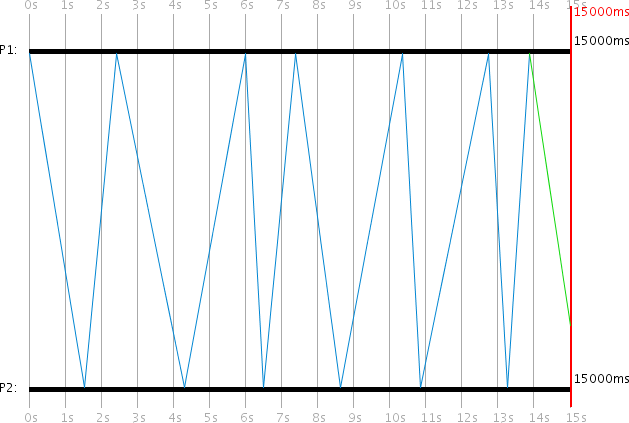
\includegraphics[width=10cm]{images/ss-protokoll-ping-pong}}
	\caption{Das Ping-Pong Protokoll}
	\label{fig:PingPongProto}
\end{figure}

Bei dem Ping-Pong Protokoll (Abbildung \ref{fig:PingPongProto}) werden zwischen zwei Prozessen, Client P1 und Server P2, st\"{a}ndig Nachrichten hin- und hergeschickt. Der Ping-Pong Client startet die erste Anfrage, worauf der Server dem Client antwortet. Auf diese Antwort wird vom Client ebenfalls geantwortet und so weiter. Jeder Nachricht wird ein Z\"{a}hler mitgeschickt, der bei jeder Station um eins inkrementiert- und jeweils im Loggfenster protokolliert wird. In Tabelle \ref{tb:PingPongTasks} sind alle f\"{u}r dieses Beispiel programmierten Ereignisse aufgef\"{u}hrt. 

\begin{figure}[h]
	\centering
	\fbox{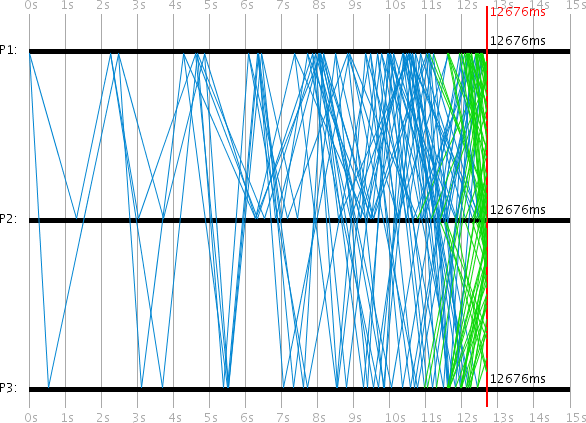
\includegraphics[width=10cm]{images/ss-protokoll-ping-pong-sturm}}
	\caption{Das Ping-Pong Protokoll (Sturm)}
	\label{fig:PingPongSturmProto}
\end{figure}

Wichtig ist, dass Prozess 1 seinen Ping-Pong Client aktiviert, bevor er eine Ping-Pong Clientanfrage startet! Wenn die Eintrittszeiten f\"{u}r die Aktivierung des Protokolls und das Starten der Anfrage identisch sind, so ordnet der Task-Manager (mehr dazu sp\"{a}ter) diese Ereignisse automatisch in der richtigen Reihenfolge an. Wenn der Ping-Pong Client nicht aktiviert werden w\"{u}rde, dann k\"{o}nnte P1 auch keine Ping-Pong Anfrage starten. Bevor ein Prozess eine Anfrage starten kann, muss er das dazugeh\"{o}rige Protokoll unterst\"{u}tzen beziehungsweise aktiviert haben. Dies gilt nat\"{u}rlich f\"{u}r alle anderen Protokolle analog. Anhand diesem Beispiel ist erkennbar, dass die noch nicht ausgelieferte Nachrichten gr\"{u}n eingef\"{a}rbt ist. Alle ausgelieferten Nachrichten tragen bereits die Farbe Blau.

Werden die Ereignisse wie in Tabelle \ref{tb:PingPongSturmTasks} abge\"{a}ndert, so l\"{a}sst sich ein Ping-Pong Sturm realisieren. Dort wurde ein neuer Prozess 3 eingef\"{u}hrt, der als zus\"{a}tzlicher Ping-Pong Server agiert. Da auf jede Clientnachricht stets zwei Serverantworten folgen, verdoppelt sich bei jedem Ping-Pong Durchgang die Anzahl der kursierenden Nachrichten. Auf Abbildung \ref{fig:PingPongSturmProto} ist der dazugeh\"{o}rige Simulationsverlauf bis zum Zeitpunkt \textit{12676ms} dargestellt.

\begin{table}
	\centering
	\fbox{
	\begin{tabular}{c|c|l}
		\textbf{Zeit (ms)} & \textbf{PID} & \textbf{Ereignis} \\
		\hline 
		 	0 & 1 & Ping Pong Client aktivieren\\
		 	0 & 2 & Ping Pong Server aktivieren\\
		 	0 & 1 & Ping Pong Clientanfrage starten
	\end{tabular}
	}
	\caption{Programmierte Ping-Pong Ereignisse}
	\label{tb:PingPongTasks}
\end{table}

\begin{table}
	\centering
	\fbox{
	\begin{tabular}{c|c|l}
		\textbf{Zeit (ms)} & \textbf{PID} & \textbf{Ereignis} \\
		\hline 
		 	0 & 1 & Ping Pong Client aktivieren\\
		 	0 & 2 & Ping Pong Server aktivieren\\
		 	0 & 3 & Ping Pong Server aktivieren\\
		 	0 & 1 & Ping Pong Clientanfrage starten
	\end{tabular}
	}
	\caption{Programmierte Ping-Pong Ereignisse (Sturm)}
	\label{tb:PingPongSturmTasks}
\end{table}

\newpage

\begin{table}
	\centering
	\fbox{
	\begin{tabular}{c|c|l}
		\textbf{Zeit (ms)} & \textbf{PID} & \textbf{Ereignis} \\
		\hline 
		 	0000 & 1 & Broadcast Client aktivieren\\
		 	0000 & 2 & Broadcast Client aktivieren\\
		 	0000 & 3 & Broadcast Client aktivieren\\
		 	0000 & 4 & Broadcast Client aktivieren\\
		 	0000 & 5 & Broadcast Client aktivieren\\
		 	0000 & 6 & Broadcast Client aktivieren\\
		 	0000 & 1 & Broadcast Server aktivieren\\
		 	0000 & 2 & Broadcast Server aktivieren\\
		 	0000 & 3 & Broadcast Server aktivieren\\
		 	0000 & 4 & Broadcast Server aktivieren\\
		 	0000 & 5 & Broadcast Server aktivieren\\
		 	0000 & 6 & Broadcast Server aktivieren\\
		 	0000 & 1 & Broadcast Clientanfrage starten\\
		 	2500 & 1 & Broadcast Clientanfrage starten
	\end{tabular}
	}
	\caption{Programmierte Broadcast Ereignisse}
	\label{tb:BroadcastSturmTasks}
\end{table}
\subsection{Das Broadcast Protokoll}

\begin{figure}[h]
	\centering
	\fbox{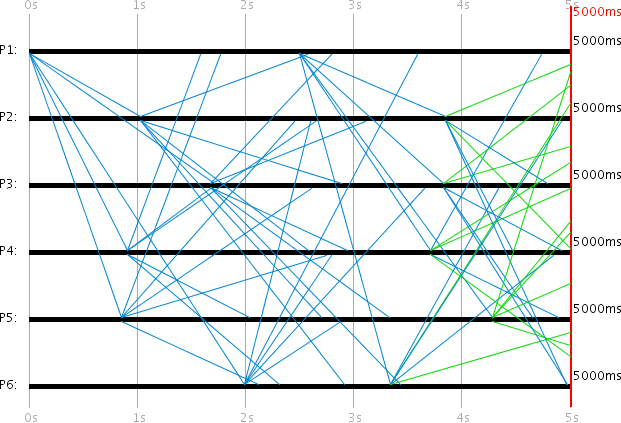
\includegraphics[width=10cm]{images/ss-protokoll-broadcast-sturm}}
	\caption{Das Broadcast Protokoll}
	\label{fig:BroadcastSturmProto}
\end{figure}

Das Broadcast Protokoll verh\"{a}lt sich \"{a}hnlich wie das Ping-Pong Protokoll. Der Unterschied besteht darin, dass sich das Protokoll anhand einer eindeutigen Broadcast-ID merkt, welche Nachrichten bereits verschickt wurden. Das Broadcast Protokoll (server- und clientseitig) verschickt alle erhaltenen Nachrichten, sofern sie vom jeweiligen Prozess noch nicht schon einmal verschickt wurden, erneut. 

Der Server und der Client unterscheiden sich in diesem Fall nicht und f\"{u}hren bei Ankunft einer Nachricht jeweis die selben Aktionen durch. Somit l\"{a}sst sich, unter Verwendung mehrerer Prozesse (hier 6), wie auf Abbildung \ref{fig:BroadcastSturmProto}, ein Broadcast erzeugen. P1 ist der Client und startet je eine Anfrage nach \textit{0ms} und \textit{2500ms}. Die Simulationsdauer betr\"{a}gt hier genau \textit{5000ms}. Da ein Client nur Servernachrichten und ein Server nur Clientnachrichten empfangen kann, ist in dieser Simulation jeder Prozess, wie in Tabelle \ref{tb:BroadcastSturmTasks} angegeben, gleichzeitig Server und Client. 

\newpage
\subsection{Das Protokoll zur internen Synchronisierung in einem synchronen System}

Bisher wurden nur Protokolle vorgef\"{u}hrt, in denen die beteiligten Prozesse keine Uhrabweichung eingestellt hatten. Das Protokoll zur internen Synchronisierung ist ein Protokoll zur Synchronisierung der lokalen Prozesszeit, welches beispielsweise angewendet werden kann, wenn eine Prozesszeit aufgrund einer Uhrabweichung falsch geht. Wenn der Client seine falsche lokale Zeit $t_c$ mit einem Server synchronisieren m\"{o}chte, so schickt er ihm eine Clientanfrage. Der Server schickt als Antwort seine eigene lokale Prozesszeit $t_s$ zur\"{u}ck, womit der Client seine neue und genauere Prozesszeit berechnen kann. Wie genau die neue Prozesszeit berechnet wird, ist im Folgenden beschrieben: 

\begin{figure}[h]
	\centering
	\fbox{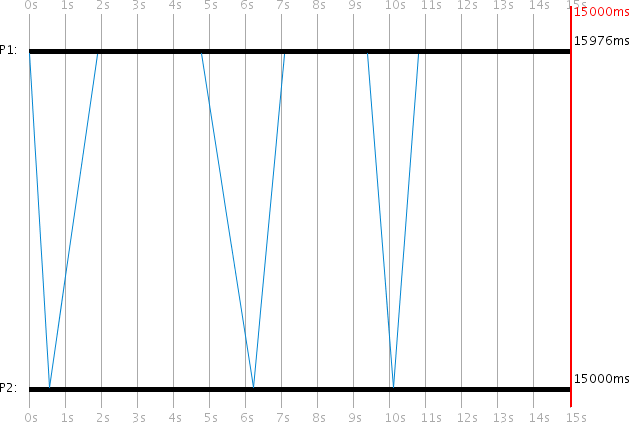
\includegraphics[width=10cm]{images/ss-protokoll-time-sync}}
	\caption{Das Protokoll zur internen Synchronisierung}
	\label{fig:TimeSyncProto}
\end{figure}

Hier (Abbildung \ref{fig:TimeSyncProto}) stellt P1 den Client und P2 den Server dar. Da die \"{U}bertragungszeit $t_u$ einer Nachricht angenommen zwischen $t'_{min}$ und $t'_{max}$ liegt, setzt der Client P1 nach Empfang der Serverantwort seine lokale Prozesszeit auf 

\begin{equation*}
	t_c := t_s + \frac{1}{2} (t'_{min} + t'_{max})
\end{equation*}

Somit wurde die lokale Zeit von P1, bis auf einen Fehler von $< \frac{1}{2} (t'_{max} - t'_{min})$, synchronisiert. 

Der Clientprozess hat in der Abbildung \ref{fig:TimeSyncProto} als Uhrabweichung den Wert \textit{0.1} und der Server hat als Uhrabweichung den Wert \textit{0.0} konfiguriert. Der Client startet, wie in Tabelle \ref{tb:InterneSyncTasks} angegeben, nach \textit{0ms}, \textit{5000ms} und \textit{10000ms} seiner lokalen Prozesszeit jeweils eine Clientanfrage. In der Abbildung l\"{a}sst sich erkennen, dass die 2. und die 3. Anfrage nicht synchron zu der globalen Zeit (siehe Sekunden-Gatter) gestartet wurden, was auf die Uhrabweichung von P1 zur\"{u}ckzuf\"{u}hren ist. Nach Simulationsende ist die Zeit von P1 bis auf \textit{15000ms} - \textit{15976ms} = \textit{-976ms} synchronisiert.

\begin{table}
	\centering
	\fbox{
	\begin{tabular}{c|c|l}
		\textbf{Zeit (ms)} & \textbf{PID} & \textbf{Ereignis} \\
		\hline 
		 	00000 & 1 & Interne Sync. Client aktivieren \\
		 	00000 & 2 & Interne Sync. Server aktivieren\\
		 	00000 & 1 & Interne Sync. Clientanfrage starten\\
		 	05000 & 1 & Interne Sync. Clientanfrage starten\\
		 	10000 & 1 & Interne Sync. Clientanfrage starten\\
	\end{tabular}
	}
	\caption{Programmierte Ereignisse zur internen Synchronisierung}
	\label{tb:InterneSyncTasks}
\end{table}

\subsubsection{Protokollvariablen}

Dieses Protokoll verwendet folgende zwei clientseitige Variablen, die in den Prozesseinstellungen unter dem Punkt ``Interne Sync. Client'' konfiguriert werden k\"{o}nnen. Serverseitig gibt es hier keine Variablen.

\begin{itemize}
	\item \textbf{Min. \"{U}bertragungszeit} \textit{(Long: 500)}: Gibt den Wert $t'_{min}$ in Millisekunden an
	\item \textbf{Max. \"{U}bertragungszeit} \textit{(Long: 2000)}: Gibt den Wert $t'_{max}$ in Millisekunden an
\end{itemize}

$t'_{min}$ und $t'_{max}$ sind die bei den Protokollberechnungen verwendeten Werte. Sie k\"{o}nnen sich allerdings von den tats\"{a}chlichen Nachrichten\"{u}bertragungszeiten $t_{min}$ und $t_{max}$ (siehe Sektion \"{u}ber Prozesseinstellungen) unterscheiden. Somit lassen sich auch Szenarien simulieren, in denen das Protokoll falsch eingestellt wurde und wo in der Zeitsynchronisierung gro�e Fehler auftreten k\"{o}nnen.

\newpage
\subsection{Christians Methode zur externen Synchronisierung}

\begin{figure}[h]
	\centering
	\fbox{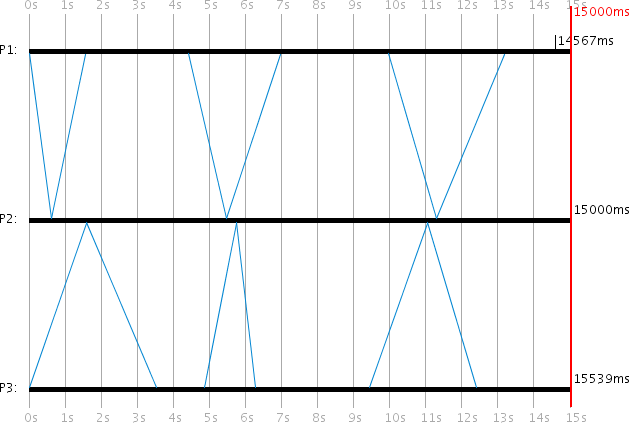
\includegraphics[width=10cm]{images/ss-protokoll-time-sync-2}}
	\caption{Interne Synchronisierung und Christians Methode im Vergleich}
	\label{fig:TimeSync2Proto}
\end{figure}

Ein weiteres Protokoll f\"{u}r die Synchronisierung von Uhrzeiten funktioniert nach der Christians Methode zur externen Synchronisierung. Die Christians Methode benutzt die RTT (Round Trip Time) $t_{rtt}$, um die \"{U}bertragungszeiten von einzelnen Nachrichten zu approximieren. 

Wenn der Client seine lokale Zeit $t_c$ bei einem Server synchronisieren m\"{o}chte, so verschickt er eine Anfrage, und misst dabei bis zur Ankunft der Serverantwort die dazugeh\"{o}rige RTT $t_{rtt}$. Die Serverantwort beinhaltet die lokale Prozesszeit $t_s$ vom Server von dem Zeitpunkt, als der Server die Antwort verschickte. Der Client setzt dann seine lokale Zeit neu auf:

\begin{equation*}
	t_c := t_s + \frac{1}{2} t_{rtt}
\end{equation*}

und zwar mit einer Genauigkeit von $\pm(\frac{1}{2} t_{rtt} - u_{min}$) wenn $u_{min}$ eine Schranke f\"{u}r eine Nachrichten\"{u}bertragung mit $t_{rtt} < u_{min}$ ist (siehe \cite{Vorlesung}).

Im Prinzip sieht ein Verlauf einer Christians-Simulation so aus wie auf Abbildung \ref{fig:TimeSyncProto}, daher wird hier auf eine einfache Abbildung vom Christians-Protokoll verzichtet. Viel Interessanter ist der direkte Vergleich zwischen dem Protokoll zur internen Synchronisierung und der Christians Methode der externen Synchronisierung (Abbildung \ref{fig:TimeSync2Proto}). Hier stellt P1 den Client zur internen Synchronisierung und P3 den Client zur externen Synchronisierung dar. P2 fungiert f\"{u}r beide Protokolle gleichzeitig als Server. P1 und P3 starten jeweils zu den lokalen Prozesszeiten \textit{0ms}, \textit{5000ms} und \textit{10000ms} eine Clientanfrage (Tabelle \ref{tb:InterneSync2Tasks}). P1 und P3 haben als Uhrabweichung \textit{0.1} eingestellt und die Simulationsdauer betr\"{a}gt insgesamt \textit{15000ms}.

Auf der Abbildung \ref{fig:TimeSync2Proto} ist ablesbar, dass nach Ablauf der Simulation P1 seine Zeit bis auf \textit{15000ms} - \textit{14567ms} = \textit{433ms} und P3 seine Zeit bis auf \textit{15000ms} - \textit{15539ms} = \textit{-539ms} synchronisiert hat. In diesem Beispiel hat also das Protokoll zur internen Synchronisierung ein besseres Ergebnis geliefert. Dies ist allerdings nicht zwingend immer der Fall, da nach einer erneuten Simulationsausf\"{u}hrung alle Nachrichten jeweils eine neue zuf\"{a}llige \"{U}bertragungszeit zwischen $t_{min}$ und $t_{max}$ haben werden, die auf das eine oder andere Protokoll wieder andere Auswirkungen haben k\"{o}nnen.

\begin{table}
	\centering
	\fbox{
	\begin{tabular}{c|c|l}
		\textbf{Zeit (ms)} & \textbf{PID} & \textbf{Ereignis} \\
		\hline 
		 	00000 & 1 & Interne Sync. Client aktivieren \\
		 	00000 & 1 & Interne Sync. Clientanfrage starten\\
		 	00000 & 2 & Christians Server aktivieren\\
		 	00000 & 2 & Interne Sync. Server aktivieren\\
		 	00000 & 3 & Christians Client aktivieren \\
		 	00000 & 3 & Christians Clientanfrage starten\\
		 	05000 & 1 & Interne Sync. Clientanfrage starten\\
		 	05000 & 3 & Christians Clientanfrage starten\\
		 	10000 & 1 & Interne Sync. Clientanfrage starten\\
		 	10000 & 3 & Christians Clientanfrage starten\\
	\end{tabular}
	}
	\caption{Programmierte Ereignisse, Vergleich interne und externe Synchronisierung}
	\label{tb:InterneSync2Tasks}
\end{table}

\newpage
\subsection{Der Berkeley Algorithmus zur internen Synchronisierung}

\begin{figure}[h]
	\centering
	\fbox{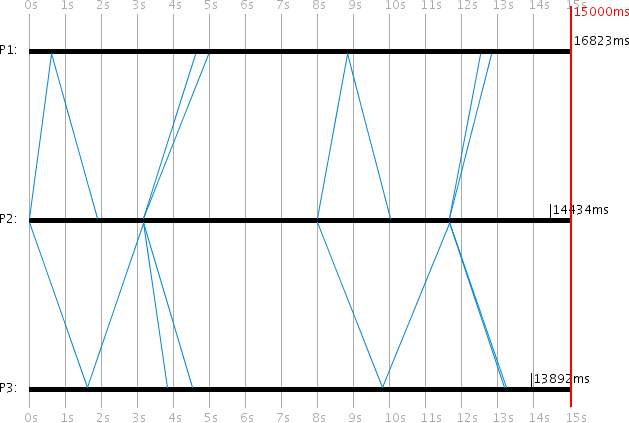
\includegraphics[width=10cm]{images/ss-protokoll-berkeley}}
	\caption{Der Berkeley Algorithmus zur internen Synchronisierung}
	\label{fig:BerkeleyProto}
\end{figure}

Der Berkeley Algorithmus zur internen Synchronisierung ist eine weitere M\"{o}glichkeit lokale Uhrzeiten abzugleichen. Dies ist das erste Protokoll, wo der Server die Anfragen startet. Der Server stellt den Koordinator des Protokolls dar. Die Clients sind somit passiv und m\"{u}ssen warten, bis eine Serveranfrage eintrifft. Hierbei muss der Server wissen, welche Clientprozesse an dem Protokoll teilnehmen, was sich in den Protokolleinstellungen des Servers einstellen l\"{a}sst.

Wenn der Server seine eigene lokale Zeit $t_s$ und auch die lokalen Prozesszeiten $t_i$ der Clients ($i = 1, ..., n$) synchronisieren m\"{o}chte, so verschickt er eine Serveranfrage. $n$ sei hierbei die Anzahl beteiligter Clients. Die Clients senden dann ihre lokalen Prozesszeiten in einer Nachricht zur\"{u}ck zum Server. Der Server hat dabei die RTTs $r_i$ bis zur Ankunft aller Clientantworten gemessen. 

Nachdem alle Antworten vorliegen, setzt er zun\"{a}chst seine eigene Zeit $t_s$ auf den Mittelwert $t_{avg}$ aller bekannten Prozesszeiten (seiner eigenen Prozesszeit eingeschlossen). Die \"{U}bertragungszeit einer Clientantwort wird auf die h\"{a}lfte der RTT gesch\"{a}tzt und wird in der Berechnung ber\"{u}cksichtigt: 

\begin{equation*}
	t_{avg} :=
	\frac{1}{n+1} ( t_s +
		\sum_{\substack{
			i=1\\
		}}^n
		\frac{r_i}{2} + t_i
	)
\end{equation*}
\begin{equation*}
	t_s := t_{avg}
\end{equation*}

Anschlie�end berechnet der Server f\"{u}r jeden Client einen Korrekturwert $k_i := t_{avg} - t_i$, den er jeweils in einer separaten Nachricht zur\"{u}ckschickt. Die Clients setzten dann jeweils die lokale Prozesszeit auf $t'_i := t'_i + k_i$. Hierbei stellt $t'_i$ die derzeit aktuelle Prozesszeit des jeweiligen Clients dar. Denn bis zum Eintreffen des Korrekturwertes ist inzwischen wieder neue Zeit verstrichen.

Im Beispiel auf Abbildung \ref{fig:BerkeleyProto} gibt es die 2 Clientprozesse P1 und P3 sowie den Serverprozess P2. Der Server startet nach jeweils \textit{0ms} und \textit{7500ms} eine Synchronisierungsanfrage (Tabelle \ref{tb:BerkeleyTasks}). Hier f\"{a}llt auf, dass der Server stets 2 Korrekturwerte verschickt, die jeweils P1 und P3 erreichen. Es werden hier also pro Synchronisierungsvorgang insgesamt 4 Korrekturwerte ausgeliefert. Eine Korrekturnachricht enth\"{a}lt neben dem Korrekturwert $k_i$ auch die PID des Prozesses, f\"{u}r den die Nachricht bestimmt ist. Indem das Protokoll die PID \"{u}berprf\"{u}ft verarbeitet ein Client so nur die f\"{u}r ihn bestimmten Korrekturwerte.

\begin{table}
	\centering
	\fbox{
	\begin{tabular}{c|c|l}
		\textbf{Zeit (ms)} & \textbf{PID} & \textbf{Ereignis} \\
		\hline 
		 	0000 & 1 & Berkeley Client aktivieren \\
		 	0000 & 2 & Berkeley Server aktivieren \\
		 	0000 & 3 & Berkeley Client aktivieren \\
		 	0000 & 2 & Berkeley Serveranfrage starten\\
		 	7500 & 2 & Berkeley Serveranfrage starten\\
	\end{tabular}
	}
	\caption{Programmierte Ereignisse zum Berkeley Algorithmus}
	\label{tb:BerkeleyTasks}
\end{table}
\subsubsection{Protokollvariablen}

Dieses Protokoll verwendet folgende serverseitige Variable, die in den Prozesseinstellungen unter dem Punkt ``Berkeley Server'' konfiguriert werden kann. Clientseitig gibt es hier keine Variablen.

\begin{itemize}
	\item \textbf{PIDs beteiliger Prozesse} \textit{(Integer[]: [1,3])}: Dieser Vektor aus Integerwerten beinhaltet alle PIDs der Berkeley Clientprozesse, mit denen der Berkeley Server die Zeit synchronisieren soll. Das Protokoll funktioniert nicht, wenn hier eine PID angegeben wird die gar nicht existiert oder nicht das Berkeley Protokoll clientseitig gar nicht unterst\"{u}tz. In diesem Fall w\"{u}rde ewig auf eine fehlende Clientantwort gewartet werden.
\end{itemize}

\newpage
\subsection{Das Ein-Phasen Commit Protokoll}

\begin{figure}[h]
	\centering
	\fbox{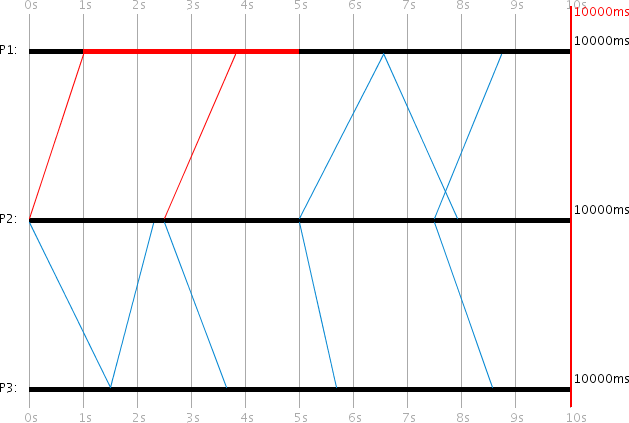
\includegraphics[width=10cm]{images/ss-protokoll-one-phase-commit}}
	\caption{Das Ein-Phasen Commit Protokoll}
	\label{fig:OnePhaseCommitProto}
\end{figure}

Das Ein-Phasen Commit Protokoll ist daf\"{u}r gedacht beliebig vielen Clients zu einer Festschreibung zu bewegen. Im realen Leben k\"{o}nnte dies beispielsweise das Erstellen oder L\"{o}schen einer Datei sein, von der auf jedem Client eine lokale Kopie existiert. Der Server ist der Koordinator und auch derjenige, der einen Festschreibewunsch initiiert. Hierbei verschickt der Server periodisch so oft den Festschreibewunsch, bis er von jedem Client eine Best\"{a}tigung erhalten hat. Der Server muss dabei die PIDs aller beteiligten Clientprozesse sowie einen Wecker f\"{u}r erneutes Versenden des Festschreibewunsches eingestellt bekommen. 

Die programmierten Ereignisse des Beispiels auf Abbildung \ref{fig:OnePhaseCommitProto} sind in Tabelle \ref{tb:OnePhaseCommitTasks} aufgelistet. P1 und P3 simulieren jeweils einen Client und P2 den Server. Damit die Simulation mehrere Festschreibew\"{u}nsche verschickt, st\"{u}rzt in der Simulation P1 nach \textit{1000ms} ab und nach \textit{5000ms} steht er wieder zur Verf\"{u}gung. Die ersten beide Festschreibew\"{u}nsche erreichen dadurch P1 nicht und erst der dritte Versuch verl\"{a}uft erfolgreich. Bevor die Best\"{a}tigung von P1 bei P2 eintrifft, l\"{a}uft jedoch der Wecker erneut ab, sodass ein weiterer Festschreibewunsch versendet wird. Da P1 und P3 jeweils schon eine Best\"{a}tigung verschickt haben, wird diese Festschreibewunschnachricht ignoriert. Jeder Client best\"{a}tigt auf einen Festschreibewunsch nur ein einziges Mal.

\begin{table}
	\centering
	\fbox{
	\begin{tabular}{c|c|l}
		\textbf{Zeit (ms)} & \textbf{PID} & \textbf{Ereignis} \\
		\hline 
		 	0000 & 1 & 1-Phasen Commit Client aktivieren\\
		 	0000 & 2 & 1-Phasen Commit Server aktivieren\\
		 	0000 & 3 & 1-Phasen Commit Client aktivieren\\
		 	0000 & 2 & 1-Phasen Commit Serveranfrage starten\\
		 	1000 & 1 & Prozessabsturz\\
		 	5000 & 1 & Prozesswiederbelebung
	\end{tabular}
	}
	\caption{Programmierte Ein-Phasen Commit Ereignisse}
	\label{tb:OnePhaseCommitTasks}
\end{table}

\subsubsection{Protokollvariablen}

Dieses Protokoll verwendet folgende serverseitige Variablen, die in den Prozesseinstellungen unter dem Punkt ``1-Phasen Commit Server'' konfiguriert werden k\"{o}nnen. Clientseitig gibt es hier keine Variablen.

\begin{itemize}
	\item \textbf{Zeit bis erneute Anfrage} \textit{(Long: timeout = 2500)}: Gibt die Anzahl von Millisekunden an, die gewartet werden sollen, bis der Festschreibewunsch erneut verschickt wird.
	\item \textbf{PIDs beteiliger Prozesse} \textit{(Integer[]: pids = [1,3])}: Dieser Vektor aus Integerwerten beinhaltet alle PIDs der Clientprozesse, die festschreiben sollen. 
\end{itemize}

\newpage
\subsection{Das Zwei-Phasen Commit Protokoll}

\begin{figure}[h]
	\centering
	\fbox{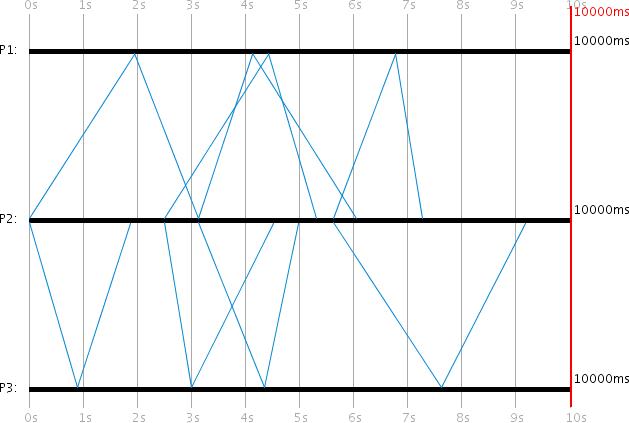
\includegraphics[width=10cm]{images/ss-protokoll-two-phase-commit}}
	\caption{Das Zwei-Phasen Commit Protokoll}
	\label{fig:TwoPhaseCommitProto}
\end{figure}

Das Zwei-Phasen Commit Protokoll ist eine Erweiterung des Ein-Phasen Commit Protokolls. Der Server startet zun\"{a}chst eine Anfrage an alle beteiligten Clients, ob festgeschrieben werden soll. Jeder Client antwortet dann mit \textit{true} oder \textit{false}. Der Server fragt so oft periodisch nach, bis alle Ergebnisse aller Clients vorliegen. Nach Erhalt aller Abstimmungen \"{u}berpr\"{u}ft der Server, ob alle mit \textit{true} abgestimmt haben. F\"{u}r den Fall dass mindestens ein Client mit \textit{false} abgestimmt hat, wird der Festschreibevorgang abgebrochen und als globales Abstimmungsergebnis \textit{false} verschickt. Wenn jedoch alle mit \textit{true} abstimmten, soll festgeschrieben werden. Dabei wird das globale Abstimmungsergebnis \textit{true} verschickt. Das globale Abstimmungsergebnis wird periodisch so oft erneut verschickt, bis von jedem Client eine Best\"{a}tigung des Erhalts vorliegt.

In dem Beispiel (Abbildung \ref{fig:TwoPhaseCommitProto}) sind P1 und P3 Clients und P2 der Server. Der Server verschickt nach \textit{0ms} seine erste Anfrage (Tabelle \ref{tb:TwoPhaseCommitTasks}). Da diese Simulation recht un\"{u}bersichtlich ist, liegen in den Tabellen \ref{tb:TwoPhaseCommitLoggs} und \ref{tb:TwoPhaseCommitLoggs2} Ausz\"{u}ge aus dem Loggfenster vor. Auf die Lamport- und Vektorzeitstempel sowie die lokalen Prozesszeiten wurde hier wegen Irrelevanz verzichtet. Da keine Uhrabweichungen konfiguriert wurden, sind die lokalen Prozesszeiten stets gleich der globalen Zeit und deswegen wird in den Tabellen pro Loggeintrag jeweils nur eine Zeit angegeben. Anhand der Nachrichten IDs lassen sich dort die einzelnen Sendungen zuordnen. In den Loggs wird auch st\"{a}ndig der Inhalt der verschickten Nachricht sowie die dazugeh\"{o}rigen Datentypen aufgef\"{u}hrt. Hier stimmen P1 und P3 jeweils mit \textit{true}, d.h. es soll festgeschrieben werden, ab. 

\begin{table}
	\centering
	\fbox{
	\begin{tabular}{c|c|l}
		\textbf{Zeit (ms)} & \textbf{PID} & \textbf{Ereignis} \\
		\hline 
		 	0000 & 1 & 2-Phasen Commit Client aktivieren\\
		 	0000 & 2 & 2-Phasen Commit Server aktivieren\\
		 	0000 & 3 & 2-Phasen Commit Client aktivieren\\
		 	0000 & 2 & 2-Phasen Commit Serveranfrage starten
	\end{tabular}
	}
	\caption{Programmierte Zwei-Phasen Commit Ereignisse}
	\label{tb:TwoPhaseCommitTasks}
\end{table}

\subsubsection{Protokollvariablen}

Dieses Protokoll verwendet folgende serverseitige Variablen, die in den Prozesseinstellungen unter dem Punkt ``2-Phasen Commit Server'' konfiguriert werden k\"{o}nnen:

\begin{itemize}
	\item \textbf{Zeit bis erneute Anfrage} \textit{(Long: timeout = 2500)}: Gibt die Anzahl von Millisekunden an, die gewartet werden sollen, bis der Festschreibewunsch erneut verschickt wird.
	\item \textbf{PIDs beteiliger Prozesse} \textit{(Integer[]: pids = [1,3])}: Dieser Vektor aus Integerwerten beinhaltet alle PIDs der Clientprozesse die \"{u}ber eine Festschreibung abstimmen und anschlie�end gegebenenfalls festschreiben sollen. 
\end{itemize}

Und folgende Clientvariable kann unter den Prozesseinstellungen unter dem Punkt ``2-Phasen Commit Client'' konfiguriert werden:

\begin{itemize}
	\item \textbf{Festschreibwahrscheinlichkeit} \textit{(Integer: ackProb = 50)}: Gibt die Wahrscheinlichkeit in Prozent an, die der Client mit \textit{true}, also f\"{u}r das Festschreiben, abstimmt.
\end{itemize}

\begin{table}
	\centering
	\fbox{
	\begin{tabular}{c|c|l}
		\textbf{Zeit (ms)} & \textbf{PID} & \textbf{Loggnachricht} \\
			\hline
000000 & & Simulation gestartet\\
\hline
000000 & 1 & 2-Phasen Commit Client aktiviert\\
\hline
000000 & 2 & 2-Phasen Commit Server aktiviert\\
\hline
000000 & 2 & Nachricht versendet; ID: 94; Protokoll: 2-Phasen Commit\\
	& & Boolean: wantVote=true\\
\hline
000000 & 3 & 2-Phasen Commit Client aktiviert\\
\hline
000905 & 3 & Nachricht erhalten; ID: 94; Protokoll: 2-Phasen Commit\\
\hline
000905 & 3 & Nachricht versendet; ID: 95; Protokoll: 2-Phasen Commit\\
	& & Integer: pid=3; Boolean: isVote=true; vote=true\\
\hline
000905 & 3 & Abstimmung true versendet\\
\hline
001880 & 2 & Nachricht erhalten; ID: 95; Protokoll: 2-Phasen Commit\\
\hline
001880 & 2 & Abstimmung von Prozess 3 erhalten! Ergebnis: true\\
\hline
001947 & 1 & Nachricht erhalten; ID: 94; Protokoll: 2-Phasen Commit\\
\hline
001947 & 1 & Nachricht versendet; ID: 96; Protokoll: 2-Phasen Commit\\
	& & Integer: pid=1; Boolean: isVote=true; vote=true\\
\hline
001947 & 1 & Abstimmung true versendet\\
\hline
002500 & 2 & Nachricht versendet; ID: 97; Protokoll: 2-Phasen Commit\\
	& & Boolean: wantVote=true\\
\hline
003006 & 3 & Nachricht erhalten; ID: 97; Protokoll: 2-Phasen Commit\\
\hline
003006 & 3 & Nachricht versendet; ID: 98; Protokoll: 2-Phasen Commit\\
	& & Integer: pid=3; Boolean: isVote=true; vote=true\\
\hline
003006 & 3 & Abstimmung true versendet\\
\hline
003137 & 2 & Nachricht erhalten; ID: 96; Protokoll: 2-Phasen Commit\\
\hline
003137 & 2 & Abstimmung von Prozess 1 erhalten! Ergebnis: true\\
\hline
003137 & 2 & Abstimmungen von allen beteiligten Prozessen erhalten!\\
	& & Globales Ergebnis: true\\
\hline
003137 & 2 & Nachricht versendet; ID: 99; Protokoll: 2-Phasen Commit\\
	& & Boolean: isVoteResult=true; voteResult=true\\
\hline
004124 & 1 & Nachricht erhalten; ID: 99; Protokoll: 2-Phasen Commit\\
\hline
004124 & 1 & Globales Abstimmungsergebnis erhalten. Ergebnis: true\\
\hline
004124 & 1 & Nachricht versendet; ID: 100; Protokoll: 2-Phasen Commit\\
	& & Integer: pid=1; Boolean: isAck=true\\
\hline
004354 & 3 & Nachricht erhalten; ID: 99; Protokoll: 2-Phasen Commit\\
\hline
004354 & 3 & Globales Abstimmungsergebnis erhalten. Ergebnis: true\\
\hline
004354 & 3 & Nachricht versendet; ID: 101; Protokoll: 2-Phasen Commit\\
	& & Integer: pid=3; Boolean: isAck=true\\
\hline
004434 & 1 & Nachricht erhalten; ID: 97; Protokoll: 2-Phasen Commit\\
\hline
004434 & 1 & Nachricht versendet; ID: 102; Protokoll: 2-Phasen Commit\\
	& & Integer: pid=1; Boolean: isVote=true; vote=true\\
	\end{tabular}
	}
	\caption{Auszug aus der Loggausgabe des Zwei-Phasen Commit Beispiels}
	\label{tb:TwoPhaseCommitLoggs}
\end{table}

\begin{table}
	\centering
	\fbox{
	\begin{tabular}{c|c|l}
		\textbf{Zeit (ms)} & \textbf{PID} & \textbf{Loggnachricht} \\
			\hline
004434 & 1 & Abstimmung true versendet\\
\hline
004527 & 2 & Nachricht erhalten; ID: 98; Protokoll: 2-Phasen Commit\\
\hline
004975 & 2 & Nachricht erhalten; ID: 101; Protokoll: 2-Phasen Commit\\
\hline
005311 & 2 & Nachricht erhalten; ID: 102; Protokoll: 2-Phasen Commit\\
\hline
005637 & 2 & Nachricht versendet; ID: 103; Protokoll: 2-Phasen Commit\\
	& & Boolean: isVoteResult=true; voteResult=true\\
\hline
006051 & 2 & Nachricht erhalten; ID: 100; Protokoll: 2-Phasen Commit\\
\hline
006051 & 2 & Alle Teilnehmer haben die Abstimmung erhalten\\
\hline
006766 & 1 & Nachricht erhalten; ID: 103; Protokoll: 2-Phasen Commit\\
\hline
006766 & 1 & Globales Abstimmungsergebnis erhalten. Ergebnis: true\\
\hline
006766 & 1 & Nachricht versendet; ID: 104; Protokoll: 2-Phasen Commit\\
	& & Integer: pid=1; Boolean: isAck=true\\
\hline
007279 & 2 & Nachricht erhalten; ID: 104; Protokoll: 2-Phasen Commit\\
\hline
007618 & 3 & Nachricht erhalten; ID: 103; Protokoll: 2-Phasen Commit\\
\hline
007618 & 3 & Globales Abstimmungsergebnis erhalten. Ergebnis: true\\
\hline
007618 & 3 & Nachricht versendet; ID: 105; Protokoll: 2-Phasen Commit\\
	& & Integer: pid=3; Boolean: isAck=true\\
\hline
009170 & 2 & Nachricht erhalten; ID: 105; Protokoll: 2-Phasen Commit\\
\hline
010000 & & Simulation beendet
	\end{tabular}
	}
	\caption{Auszug aus der Loggausgabe des Zwei-Phasen Commit Beispiels (2)}
	\label{tb:TwoPhaseCommitLoggs2}
\end{table}

\newpage
\subsection{Der ungen\"{u}gende (Basic) Multicast}

\begin{figure}[h]
	\centering
	\fbox{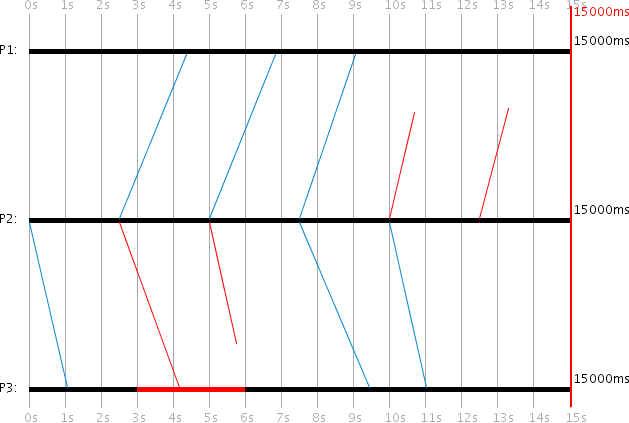
\includegraphics[width=10cm]{images/ss-protokoll-basic-multicast}}
	\caption{Das Basic-Multicast Protokoll}
	\label{fig:BasicMulticastProto}
\end{figure}

Das Basic-Multicast Protokoll ist sehr einfach aufgebaut. Im Beispiel auf Abbildung \ref{fig:BasicMulticastProto} sind P1 und P3 Server und P2 der Client. Bei diesem Protokoll startet der Client immer die Anfrage, welche bei diesem Protokoll eine einfache Multicast-Nachricht darstellen soll. Die Basic-Multicast Server dienen lediglich f\"{u}r den Empfang einer Nachricht. Es werden keine Best\"{a}tigungen verschickt. Wie in Tabelle \ref{tb:BasicMulticastTasks} aufgef\"{u}hrt verschickt P2 alle \textit{2500ms} jeweils eine Multicast-Nachricht, die alle voneinander v\"{o}llig unabh\"{a}ngig sind. 

P1 kann jedoch erst nach \textit{2500ms} Multicast-Nachrichten empfangen, da er vorher das Protokoll nicht unterst\"{u}tzt w\"{a}hrend P3 von \textit{3000ms} bis \textit{6000ms} abgest\"{u}rzt ist und in dieser Zeit auch keine Nachrichten empfangen kann. Je nach Interpretation k\"{o}nnte P1 einen Server simulieren, der erst sp\"{a}ter ans Netz angeschlossen wird. Da die Einstellung ``Nur relevante Nachrichten anzeigen'' aktiviert ist, wird die erste Multicast-Nachricht von P2 an P1 nicht dargestellt. Bei jedem Prozess wurde die Nachrichtenverlustwahrscheinlichkeit auf \textit{30} Prozent gestellt, weswegen alle in dieser Simulation verschickten Nachrichten mit einer Wahrscheinlichkeit von \textit{30} Prozent ausfallen. 

In diesem Beispiel ging die 3. Multicast-Nachricht auf den Weg zu P3- und die 5. sowie 6. Nachricht auf den Weg zu P1 verloren. Lediglich die 4. Multicast-Nachricht hat alle beiden Ziele aufeinmal erreicht.

\begin{table}
	\centering
	\fbox{
	\begin{tabular}{c|c|l}
		\textbf{Zeit (ms)} & \textbf{PID} & \textbf{Ereignis} \\
		\hline 
		 	00000 & 2 & Basic Multicast Client aktivieren\\
		 	00000 & 3 & Basic Multicast Server aktivieren\\
		 	00000 & 2 & Basic Multicast Clientanfrage starten\\
		 	02500 & 1 & Basic Multicast Server aktivieren\\
		 	02500 & 2 & Basic Multicast Clientanfrage starten\\
		 	03000 & 3 & Prozessabsturz\\
		 	05000 & 2 & Basic Multicast Clientanfrage starten\\
		 	06000 & 3 & Prozesswiederbelebung\\
		 	07500 & 2 & Basic Multicast Clientanfrage starten\\
		 	10000 & 2 & Basic Multicast Clientanfrage starten\\
		 	12500 & 2 & Basic Multicast Clientanfrage starten
	\end{tabular}
	}
	\caption{Programmierte Basic-Multicast Ereignisse}
	\label{tb:BasicMulticastTasks}
\end{table}

\newpage
\subsection{Der zuverl\"{a}ssige (Reliable) Multicast}

\begin{figure}[h]
	\centering
	\fbox{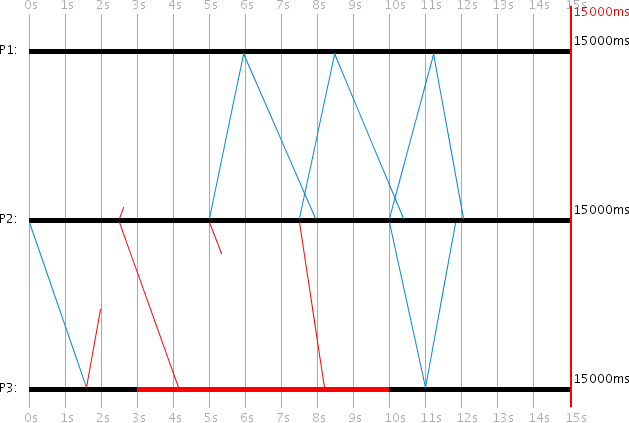
\includegraphics[width=10cm]{images/ss-protokoll-reliable-multicast}}
	\caption{Das Reliable-Multicast Protokoll}
	\label{fig:ReliableMulticastProto}
\end{figure}

Bei dem  zuverl\"{a}ssigen (Reliable) Multicast verschickt der Client so oft periodisch seine Multicast-Nachricht erneut, bis er von allen beteiligten Servern eine Best\"{a}tigung erhalten hat. Nach jedem erneuten Versuch vergisst der Client, von welchen Servern er bereits eine Best\"{a}tigung erhalten hat, womit jeder erneuter Versuch von allen Teilnehmern aufs Neue best\"{a}tigt werden muss. In dem Beispiel (Abbildung \ref{fig:ReliableMulticastProto}, Tabelle \ref{tb:ReliableMulticastTasks}, sowie den Loggs in den Tabellen \ref{tb:ReliableMulticastLoggs} und \ref{tb:ReliableMulticastLoggs2}) ist P2 der Multicast-verschickende Client, w\"{a}hrend P1 und P3 die Server darstellen. Bei \textit{0ms} initiiert der Client seine Multicast-Nachricht. Die Nachrichtenverlustwahrscheinlichkeiten sind bei allen Prozessen auf \textit{30} Prozent eingestellt.

In diesem Beispiel ben\"{o}tigt der Client bis zur erfolgreichen Auslieferung des zuverl\"{a}ssigen Multicasts genau 5 Versuche:

\begin{enumerate}
	\setlength{\itemsep}{-1mm}
	\item Versuch: 
		\begin{itemize}
			\setlength{\itemsep}{-2.5mm}
			\item P1 unterst\"{u}tzt das Reliable-Multicast Protokoll noch nicht, und kann somit weder Multicast-Nachricht erhalten noch eine Best\"{a}tigung verschicken.
			\item P3 empf\"{a}ngt die Multicast-Nachricht, jedoch geht seine Best\"{a}tigungsnachricht verloren.
		\end{itemize}
	\item Versuch: 
		\begin{itemize}
			\setlength{\itemsep}{-2.5mm}
			\item P1: Die Multicast-Nachricht geht unterwegs zu P1 verloren.
			\item P3: Die Multicast-Nachricht erreicht P3, aber P3 ist abgest\"{u}rzt und kann somit keine Nachricht verarbeiten.
		\end{itemize}
	\item Versuch: 
		\begin{itemize}
			\setlength{\itemsep}{-2.5mm}
			\item P1 empf\"{a}ngt die Multicast-Nachricht und seine Best\"{a}tigung kommt wie geplant bei P2 an. 
			\item P3: Die Multicast-Nachricht geht unterwegs zu P3 verloren.
		\end{itemize}
	\item Versuch: 
		\begin{itemize}
			\setlength{\itemsep}{-2.5mm}
			\item P1 empf\"{a}ngt die Multicast-Nachricht und seine Best\"{a}tigung kommt wie geplant bei P2 an. 
			\item P3: Die Multicast-Nachricht erreicht P3, aber P3 ist abgest\"{u}rzt und kann somit keine Nachricht verarbeiten.
		\end{itemize}
	\item Versuch: 
		\begin{itemize}
			\item P1 empf\"{a}ngt die Multicast-Nachricht und seine Best\"{a}tigung kommt wie geplant bei P2 an. 
			\setlength{\itemsep}{-2.5mm}
			\item P3 empf\"{a}ngt die Multicast-Nachricht und seine Best\"{a}tigung kommt wie geplant bei P2 an. 
		\end{itemize}
\end{enumerate}

\begin{table}
	\centering
	\fbox{
	\begin{tabular}{c|c|l}
		\textbf{Zeit (ms)} & \textbf{PID} & \textbf{Ereignis} \\
		\hline 
		 	00000 & 3 & Reliable Multicast Server aktivieren\\
		 	00000 & 2 & Reliable Multicast Client aktivieren\\
		 	00000 & 2 & Reliable Multicast Clientanfrage starten\\
		 	02500 & 1 & Reliable Multicast Server aktivieren\\
		 	03000 & 3 & Prozessabsturz\\
		 	10000 & 3 & Prozesswiederbelebung\\
	\end{tabular}
	}
	\caption{Programmierte Reliable-Multicast Ereignisse}
	\label{tb:ReliableMulticastTasks}
\end{table}

\begin{table}
	\centering
	\fbox{
	\begin{tabular}{c|c|l}
		\textbf{Zeit (ms)} & \textbf{PID} & \textbf{Loggnachricht} \\
			\hline
000000 & & Simulation gestartet\\
\hline
000000 & 2 & Reliable Multicast Client aktiviert\\
\hline
000000 & 2 & Nachricht versendet; ID: 280; Protokoll: Reliable Multicast;\\
	   & & Boolean: isMulticast=true\\
\hline
000000 & 3 & Reliable Multicast Server aktiviert\\
\hline
001590 & 3 & Nachricht erhalten; ID: 280; Protokoll: Reliable Multicast\\
\hline
001590 & 3 & Nachricht versendet; ID: 281; Protokoll: Reliable Multicast\\
	   & & Integer: pid=3; Boolean: isAck=true\\
\hline
001590 & 3 & ACK versendet\\
\hline
002500 & 1 & Reliable Multicast Server aktiviert\\
\hline
002500 & 2 & Nachricht versendet; ID: 282; Protokoll: Reliable Multicast\\
	   & & Boolean: isMulticast=true\\
\hline
003000 & 3 & Abgest�rzt\\
\hline
005000 & 2 & Nachricht versendet; ID: 283; Protokoll: Reliable Multicast\\
	   & & Boolean: isMulticast=true\\
\hline
005952 & 1 & Nachricht erhalten; ID: 283; Protokoll: Reliable Multicast\\
\hline
005952 & 1 & Nachricht versendet; ID: 284; Protokoll: Reliable Multicast\\
	   & & Integer: pid=1; Boolean: isAck=true\\
\hline
005952 & 1 & ACK versendet\\
\hline
007500 & 2 & Nachricht versendet; ID: 285; Protokoll: Reliable Multicast\\
	   & & Boolean: isMulticast=true\\
\hline
007937 & 2 & Nachricht erhalten; ID: 284; Protokoll: Reliable Multicast\\
\hline
007937 & 2 & ACK von Prozess 1 erhalten!\\
\hline
008469 & 1 & Nachricht erhalten; ID: 285; Protokoll: Reliable Multicast\\
\hline
008469 & 1 & Nachricht versendet; ID: 286; Protokoll: Reliable Multicast\\
	   & & Integer: pid=1; Boolean: isAck=true\\
\hline
008469 & 1 & ACK erneut versendet\\
\hline
010000 & 2 & Nachricht versendet; ID: 287; Protokoll: Reliable Multicast\\
	   & & Boolean: isMulticast=true\\
\hline
010000 & 3 & Wiederbelebt\\
\hline
010395 & 2 & Nachricht erhalten; ID: 286; Protokoll: Reliable Multicast\\
\hline
010995 & 3 & Nachricht erhalten; ID: 287; Protokoll: Reliable Multicast\\
\hline
010995 & 3 & Nachricht versendet; ID: 288; Protokoll: Reliable Multicast\\
	   & & Integer: pid=3; Boolean: isAck=true\\
\hline
010995 & 3 & ACK erneut versendet\\
\hline
011213 & 1 & Nachricht erhalten; ID: 287; Protokoll: Reliable Multicast\\
\hline
011213 & 1 & Nachricht versendet; ID: 289; Protokoll: Reliable Multicast\\
	   & & Integer: pid=1; Boolean: isAck=true\\
	\end{tabular}
	}
	\caption{Auszug aus der Loggausgabe des Reliable-Multicast Beispiels}
	\label{tb:ReliableMulticastLoggs}
\end{table}

\begin{table}
	\centering
	\fbox{
	\begin{tabular}{c|c|l}
		\textbf{Zeit (ms)} & \textbf{PID} & \textbf{Loggnachricht} \\
			\hline
011213 & 1 & ACK erneut versendet\\
\hline
011813 & 2 &  Nachricht erhalten; ID: 288; Protokoll: Reliable Multicast\\
\hline
011813 & 2 &  ACK von Prozess 3 erhalten!\\
\hline
011813 & 2 &  ACKs von allen beteiligten Prozessen erhalten!\\
\hline
012047 & 2 &  Nachricht erhalten; ID: 289; Protokoll: Reliable Multicast\\
\hline
015000 & & Simulation beendet\\
	\end{tabular}
	}
	\caption{Auszug aus der Loggausgabe des Reliable-Multicast Beispiels (2)}
	\label{tb:ReliableMulticastLoggs2}
\end{table}

\subsubsection{Protokollvariablen}

Dieses Protokoll verwendet folgende serverseitige Variablen, die in den Prozesseinstellungen unter dem Punkt ``Reliable Multicast Server'' konfiguriert werden k\"{o}nnen:

\begin{itemize}
	\item \textbf{Zeit bis erneute Anfrage} \textit{(Long: timeout = 2500)}: Gibt die Anzahl von Millisekunden an, die gewartet werden sollen, bis der Muticast erneut verschickt wird.
	\item \textbf{PIDs beteiliger Prozesse} \textit{(Integer[]: pids = [1,3])}: Dieser Vektor aus Integerwerten beinhaltet alle PIDs der Serverprozesse, die die Multicast-Nachricht erhalten sollen.
\end{itemize}

\newpage
\section{Weitere Beispiele}

Bisher wurden alle verf\"{u}gbaren Protokolle anhand von Beispielen aufgef\"{u}hrt. Mit dem Simulator lassen sich allerdings noch viel mehr Szenarien simulieren. Daher soll hier auf weitere Anwendungsbeispiele eingegangen werden.

\subsection{Simulation von Vektor- und Lamportzeitstempel}

\begin{figure}[h]
	\centering
	\fbox{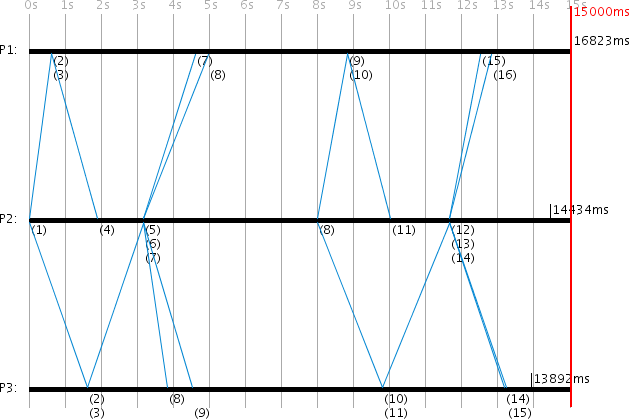
\includegraphics[width=10cm]{images/ss-protokoll-berkeley-lamport}}
	\caption{Lamportzeitstempel}
	\label{fig:Lamportzeit}
\end{figure}

Die Vektor- und Lamportzeitstempel lassen sich sehr gut am bereits behandeltem Beispiel des Berkeley-Protokoll's demonstrieren. Nach Aktivierung des Lamportzeit-Schalters erscheint bei jedem Ereignis eines Prozesses der aktuelle Lamportzeitstempel (Abbildung \ref{fig:Lamportzeit}). Jeder Prozess besitzt einen eigenen Lamportzeitstempel, der bei jedem Versenden oder Erhalten einer Nachricht inkrementiert wird. Jeder Nachricht wird die aktuelle Lamportzeit $t_l(i)$ des Senderprozesses $i$ beigef\"{u}gt. Wenn ein weiterer Prozess $j$ diese Nachricht erh\"{a}lt, so wird der aktuelle Lamportzeitstempel $t_l(j)$ von Prozess $j$ wie folgt neu berechnet:

\begin{equation*}
	t_l(j) := 1 + max(t_l(j), t_l(i))
\end{equation*}

Es wird also stets die gr\"{o}ssere Lamportzeit vom Sender- und Empf\"{a}ngerprozess verwendet und anschlie�end wird diese um \textit{1} inkrementiert. Nach Ablauf der Berkeley-Simulation hat P1 \textit{(16)}, P2 (\textit{14}) und P3 (\textit{15}) als Lamportzeitstempel abgespeichert. 

\begin{figure}[h]
	\centering
	\fbox{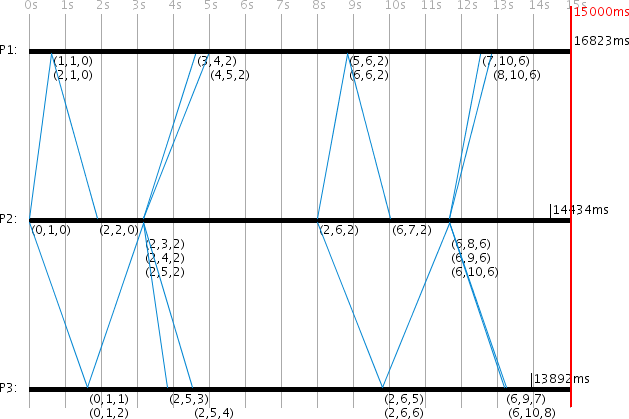
\includegraphics[width=10cm]{images/ss-protokoll-berkeley-vektor}}
	\caption{Vektorzeitstempel}
	\label{fig:Vektorzeit}
\end{figure}

Mit aktiven Vektorzeit-Schalter werden alle Vektor-Zeitstempel angezeigt (Abbildung \ref{fig:Vektorzeit}). Wie bei den Lamportzeitstempeln wird auch hier jeder Nachricht der aktuelle Vektor-Zeitstempel des Senderprozesses beigegef\"{u}gt. Bei $n$ beteiligten Prozessen hat der Vektor-Zeitstempel $v$ die gr\"{o}�e $n$. Somit gibt es f\"{u}r jeden beteiligten Prozess $i$ einen eigenen Index $i$. \"{U}ber $v(i)$ kann jeder Prozess auf seinen lokalen Eintrag zugreifen. 

Standardm\"{a}�ig wird der Vektor-Zeitstempel nur inkrementiert, wenn eine Nachricht verschickt- oder erhalten wird. Bei beiden F\"{a}llen inkrementiert der Sender- und Empf\"{a}ngerprozess jeweils seinen eigenen Index im Vektor-Zeitstempel mit $v(i) = v(i) + 1$. Beim Empfang einer Nachricht wird anschlie�end der lokale Vektor-Zeitstempel mit dem des Senderprozesses verglichen und f\"{u}r alle Indizies stets der gr\"{o}�ere Wert in den lokalen Vektor-Zeitstempel \"{u}bernommen.

Im Beispiel auf Abbildung \ref{fig:Vektorzeit} hat P1 \textit{(8,10,6)}, P2 \textit{(6,10,6)} und P3 \textit{(6,10,8)} als Vektor-Zeitstempel abgespeichert.

Wenn im Laufe einer Simulation Prozesse entfernt- oder neue Prozesse hinzugef\"{u}gt werden, so passt sich die Gr\"{o}�e der Vektor-Zeitstempel aller anderen Prozesse automatisch der Anzahl der Prozesse an.

Wie bereits beschrieben gibt es in den Simulationseinstellungen die boolschen Variablen ``Lamportzeiten betreffen alle Ereignisse'' und ``Vektorzeiten betreffen alle Ereignisse'', die standardm\"{a}�ig auf \textit{false} gesetzt sind. Mit \textit{true} werden alle Ereignisse, und nicht nur der Empfang oder das Versenden einer Nachricht, ber\"{u}cksichtigt. F\"{u}r eine weitere Betrachtung der Lamport- sowie Vektor-Zeitstempel siehe \cite{Vorlesung} oder \cite{Tanenbaum}.

\newpage
\subsection{Simulation langsamer Verbindungen}

Mit dem Simulator lassen sich auch langsame Verbindungen zu einem bestimmten Prozess simulieren. F\"{u}r die Demonstration wird das Beispiel aus Kapitel 2.5.5 wieder aufgegriffen, wo das Protokoll zur internen Synchronisation (P1) mit der Christians-Methode (P3) parallel simuliert wurden. P2 stellt den Server beider Protokolle zur Verf\"{u}gung. In diesem Szenario soll P3 eine schlechte Netzwerkverbindung besitzen, sodass Nachrichten von- und an P3 stets eine l\"{a}ngere \"{U}bertragungszeit ben\"{o}tigen.

Die Ereignisse sind so wie bereits auf Tabelle \ref{tb:InterneSync2Tasks} dargestellt wurde programmiert. In den Simulationseinstellungen ist hier die Einstellung ``Mittelwerte der \"{U}bertragungszeiten bilden'' aktiviert. In den Prozesseinstellungen von P3 wurde ``Minimale \"{U}bertragungszeit'' auf \textit{2000ms} und ``Maximale \"{U}bertragungszeit'' auf \textit{8000ms} gesetzt. P1 und P2 behalten als Standardeinstellungen f\"{u}r die minimale und maximale \"{U}bertragungszeiten jeweils \textit{500ms} und \textit{2000ms} eingestellt. Die Simulationsdauer wurde auf \textit{20000ms} gesetzt.

\begin{figure}[h]
	\centering
	\fbox{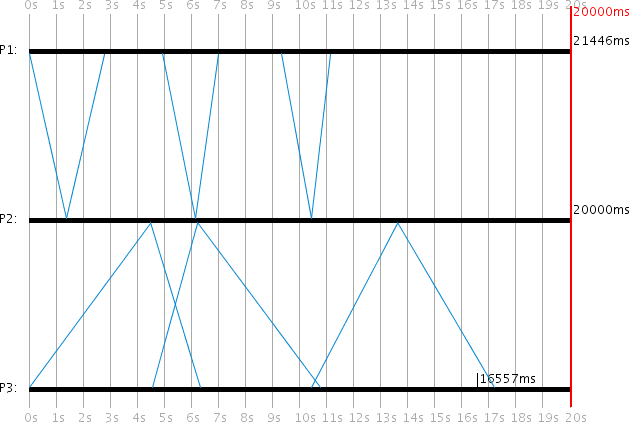
\includegraphics[width=10cm]{images/ss-protokoll-time-sync-2-long-transfer}}
	\caption{Simulation einer langsamen Verbindung}
	\label{fig:TimeSync2LongTransferProto}
\end{figure}

Als Folge (Abbildung \ref{fig:TimeSync2LongTransferProto}) dauern Nachrichten, die von- und an P3 verschickt werden, f\"{u}r eine \"{U}bertragung immer l\"{a}nger. Bevor P3 eine Antwort auf seine vorherige Anfrage bekommt, verschickt er eine erneute Anfrage. Da P3 die Serverantworten immer stets seiner letzten verschickten Anfrage zuordnet, berechnet er die RTTs allesamt falsch und seine lokale Zeit wird bei jedem Durchgang zus\"{a}tzlich verf\"{a}lscht. Die Berechnungsformeln der \"{U}bertragungszeiten wurde bereits in Kapitel 2.4.3 bei den Prozesseinstellungen behandelt. Konkret bedeutet dies f\"{u}r die \"{U}bertragungszeiten alle Nachrichten von- und an P3 jeweils:

\begin{equation*}
	\frac{1}{2} (rand(500, 2000) + rand(2000, 8000)) = \frac{1}{2} rand(2500, 10000) = rand(1250, 5000) ms
\end{equation*}
